%%%%%%%%%%%%%%%%%%%%%%%%%%%%%%%%%%%%%%%%%%%%%%%%%%%%%%%%%%%%%%%%%%%%%%%%%%%%%%%%%%%%%
%                        Author: Harshit Prashant Dhanwalkar                        %
%%%%%%%%%%%%%%%%%%%%%%%%%%%%%%%%%%%%%%%%%%%%%%%%%%%%%%%%%%%%%%%%%%%%%%%%%%%%%%%%%%%%%

%-------------------------------------------------------------------------------------
%                    PACKAGES AND OTHER DOCUMENT CONFIGURATIONS                      %
%-------------------------------------------------------------------------------------
\documentclass[fleqn,10pt]{SelfArx} % Document font size and equations flushed left
\usepackage[english]{babel} 
\usepackage{enumitem}

\usepackage{tikz}
\usetikzlibrary{trees, positioning}
\usetikzlibrary{shapes, shadings}
\usepackage{tikz-3dplot}
\usetikzlibrary{3d,shapes.geometric,shadows.blur}
\tikzstyle{vertex}=[draw,fill=black!15,circle,minimum size=20pt,inner sep=0pt]
\tikzstyle{selected edge} = [draw,line width=5pt,-,red!50]

\usepackage{amsmath}
\usepackage{array} % for tables


\usepackage{mathtools}

% \usepackage[table,xcdraw]{xcolor}
% \usepackage[table, dvipsnames]{xcolor}

\usepackage{pgfplots}
\pgfplotsset{compat=1.18}
\tdplotsetmaincoords{60}{115}
\pgfplotsset{compat=newest}

\usepackage{subfig}

%-------------------------------------------------------------------------------------
%                                       COLUMNS                                      %
%-------------------------------------------------------------------------------------
\setlength{\columnsep}{0.55cm} % Distance between the two columns of text
\setlength{\fboxrule}{0.75pt} % Width of the border around the abstract

%-------------------------------------------------------------------------------------
%                                        COLORS                                      %
%-------------------------------------------------------------------------------------
\definecolor{color1}{RGB}{0,0,90} % Color of the article title and sections
\definecolor{color2}{RGB}{0,20,20} % Color of the boxes behind the abstract and headings

%-------------------------------------------------------------------------------------
%                                       EQUATIONS                                    %
%-------------------------------------------------------------------------------------
\usepackage{cancel} % for crossing the word showing it is cancelled or is zero

%-------------------------------------------------------------------------------------
%                                     EQUATIONLINKS                                  %
%-------------------------------------------------------------------------------------
\newcommand{\myeqref}[1]{Eq.\textcolor{blue}{\textup{(\getrefnumber{#1})}}}

%-------------------------------------------------------------------------------------
%                                       HYPERLINKS                                   %
%-------------------------------------------------------------------------------------
\usepackage{xcolor}
\usepackage{hyperref}
\usepackage{footnote}

%\newcommand{\myhref}[2]{\href{#1}{\textcolor{blue}{#2}}}
\newcommand{\myhref}[2]{%
  \href{#1}{\textcolor{blue}{#2}}%
  \footnote{\url{#1}}%
}

\usepackage{cleveref}
% Customize cleveref to use "Eq." for equations
\crefname{equation}{Eq.}{Eq.}
\Crefname{equation}{Eq.}{Eq.}

\hypersetup{
	hidelinks,
	colorlinks,
	breaklinks=true,
	urlcolor=color2,
	citecolor=color1,
	linkcolor=color1,
	bookmarksopen=false,
	pdftitle={Title},
	pdfauthor={Author},
}

% ------------------------------------------------------------------------------------
%                                       CUSTOM  SYMBOLS                              %
%-------------------------------------------------------------------------------------
\newcommand{\zbar}{\raisebox{0.2ex}{--}\kern-0.6em Z}

% ------------------------------------------------------------------------------------
%                                       CUSTOM  YELLOW STICKY NOTES		     %
%-------------------------------------------------------------------------------------
\usepackage{color, colortbl}
\usepackage{calc}

\setlength{\parskip}{0ex}
\setlength{\parindent}{0ex}

\newlength{\yellownotewidth}
\setlength{\yellownotewidth}{2.5cm}
\newlength{\yellownoteheight}
\setlength{\yellownoteheight}{2.5cm}

% Yellow note...
\newcommand{\yellownote}[1]{
    \vspace{0.2\yellownoteheight}
        \begin{center}
        \begin{tikzpicture}
            % Shadow effect
            \draw[white,fill=gray!70,opacity=0.75,shift={(-0.15,-0.15)}]
		    (0,0) -- (0.07, \yellownoteheight) -- (\yellownotewidth + 0.05, \yellownoteheight) -- (2.5, 0.4) -- (2.2,0.18) -- (2, 0) -- cycle;
            % Yellow note background
	    \draw[fill=yellow!35]
		    (0,0) -- (0, \yellownoteheight) -- (\yellownotewidth, \yellownoteheight) -- (2.5, 0.4) -- (2.1,0.2) -- (1.7, 0) -- cycle;
            % Folded corner
            \draw[opacity=0.45,fill=gray!50] (0.7\yellownotewidth,0) -- 
                (0.9\yellownotewidth,0.45) -- (\yellownotewidth,0.4) -- cycle;
            % Note content
            \node[blue,below] at (0.5\yellownotewidth,\yellownoteheight) {
                \begin{minipage}{\yellownotewidth-1em}
                    \scriptsize\sf#1
                \end{minipage}
            };
        \end{tikzpicture}
        \end{center}
}

% Floating yellow note
\newcommand{\freeyellownote}[3]{
    \begin{tikzpicture}[remember picture,overlay]
        \node[anchor=north west, xshift=#1, yshift=#2] at (current page.north west) {
            \begin{tikzpicture}
            % Shadow effect
            \draw[white,fill=gray!70,opacity=0.75,shift={(-0.15,-0.15)}]
		    (0,0) -- (0.07, \yellownoteheight) -- (\yellownotewidth + 0.05, \yellownoteheight) -- (2.5, 0.4) -- (2.2,0.18) -- (2, 0) -- cycle;
            % Yellow note background
	    \draw[fill=yellow!35]
		    (0,0) -- (0, \yellownoteheight) -- (\yellownotewidth, \yellownoteheight) -- (2.5, 0.4) -- (2.1,0.2) -- (1.7, 0) -- cycle;
                % Folded corner
                \draw[opacity=0.45,fill=gray!50] 
                    (0.7\yellownotewidth,0) -- 
                    (0.9\yellownotewidth,0.45) -- 
                    (\yellownotewidth,0.4) -- 
                    cycle;
                % Note content
                \node[blue,below] at (0.5\yellownotewidth,\yellownoteheight) {
                    \begin{minipage}{\yellownotewidth-1em}
                        \scriptsize\sf#3
                    \end{minipage}
                };
            \end{tikzpicture}
        };
    \end{tikzpicture}
}

\definecolor{LightCyan}{rgb}{0.88,1,1}

%-------------------------------------------------------------------------------------
%                                       FRACTION WITHOUT FRACTION BAR                %
%-------------------------------------------------------------------------------------
\newcommand*{\bfrac}[2]{\genfrac{}{}{0pt}{}{#1}{#2}}
%-------------------------------------------------------------------------------------

%-------------------------------------------------------------------------------------
%                                       ARTICLE INFORMATION                          %
%-------------------------------------------------------------------------------------
\JournalInfo{Dual Degree Engineering Physics, 8$^{th}$ Semester, 2024} % Journal information
\Archive{Mtech, Earth System Sciences (ESS), 1$^{st}$ year} % Additional notes (e.g. copyright, DOI, review/research article)

\PaperTitle{Lecture Notes on Numerical Weather Prediction} % Article title

\Authors{Harshit Prashant Dhanwalkar (SC21B164)\textsuperscript{1}*} % Authors
\affiliation{\textsuperscript{1}\textit{MTech, Earth System Sciences (ESS), 1$^{st}$ year, Department of Physics, Indian Institute Of Spacescience and Technology (IIST)}} % Author affiliation
\affiliation{*\textbf{email}: harshitpd1729@gamil.com}

\newcommand{\keywordname}{Keywords} % Defines the keywords heading name
\Keywords{}

%-------------------------------------------------------------------------------------
%                                           ABSTRACT                                 %
%-------------------------------------------------------------------------------------
\Abstract{Notes of Lectures and addional information from books.}

%-------------------------------------------------------------------------------------
%                                            DOCUMENT                                %
%-------------------------------------------------------------------------------------
\begin{document}
\maketitle % Output the title and abstract box
\thispagestyle{empty} % Removes page number
\clearpage

\begingroup
\thispagestyle{empty} % No page number
\tableofcontents
\endgroup
\newpage

\begingroup
\thispagestyle{empty} % No page number
\listoffigures
\clearpage
\endgroup
\newpage

%-------------------------------------------------------------------------------------
%                                       DOCUMENT CONTENTS                           %
%-------------------------------------------------------------------------------------
%\addcontentsline{toc}{section}{Introduction} % Adds this section to the table of contents
%-------------------------------------------------------------------------------------
\section{Lecture 1 06/01/2025}
\subsection{Introduction to Numerical Weather Prediction}
Numerical Weathering Problem (NWP) was first proposed by Bjerkives around 1900. It is mathematical initial value problem (IVP).

Initial value Problem (IVP) $\rightarrow$ simple pendulum.
\begin{align*}
	\ddot{\theta} + \omega^2 \theta          & = 0 \tag{1.1} \label{eq:simplependulum1}                                          \\
	\frac{d^2\theta}{dt^2} + \omega^2 \theta & = 0 \tag{1.2} \label{eq:simplependulum2}                                          \\
	\theta(t)                                & = A \cos(\omega t) + B \sin(\omega t) \tag{1.3} \label{eq:simplependulumsolution}
\end{align*}

\myeqref{eq:simplependulum1} and \myeqref{eq:simplependulum2} are second order linear ordinary differential equation, whose solution .\myeqref{eq:simplependulumsolution} has 2 constants of integration $A$ and $B$. Here $\theta$ and $t$ are the dependent and independent variable since \myeqref{eq:simplependulum1} and \myeqref{eq:simplependulum2} have only one independent variable.

Values of $A$ and $B$ will depend on initial condition.

Since ODE is second order, 2 initial condition are needed at initial time, say $t=0$. Which are:
\begin{align*}
	\begin{rcases}
		\theta(t=0) = 1 \\
		\frac{\theta(t=0)}{dt} = 0
	\end{rcases} & \tag{1.4} \label{eq:att=0}
\end{align*}

\myeqref{eq:simplependulum2} and initial conditions \myeqref{eq:att=0} are together called \textbf{Mathematical IVP}. For any physical system the following two requirements are needed:
\begin{enumerate}[noitemsep]
	\item The equation (ODE or PDE) that governs the evolution of the above system.
	\item The initial state of the system.
\end{enumerate}

7 independent variables \textbf{(u,v,w,T,$\boldsymbol{\rho}$,p,q)}.

Surface area of Earth = $4\pi R^2$ = $4\pi (6.37 \times 10^{12})$ $\approx 5.1 \times 10^{14}$ m$^2$
%-------------------------------------------------------------------------------------
\clearpage
%-------------------------------------------------------------------------------------
\section{Lecture 2 07/01/2025}
7 independent variables \textbf{(u,v,w,T,$\boldsymbol{\rho}$,p,q)} therefore we need 7 Governing equations (system of 7 coupled non-linear partial differential equations):
\begin{enumerate}[noitemsep]
	\item Conservation of masss (continuity equation).
	\item Conservation of momentum in rotating frame of refrence (3 scalar equations, one each corresponding to scalar component of velocity).
	\item Conservation of energy (Thermodynamic energy equation).
	\item Conservation of moisture (moisture continuity equation).
	\item Equation of state (Ideal gas equation).
\end{enumerate}

Euler discription of fluid motion is more convinent becasue of dependence on time and above 7 equations.

Total advective and convective time of lagrangian is given by:
\begin{align*}
	\underbrace{\frac{DT}{Dt}}_\text{Lagrangian Derivative} & = \underbrace{\underbrace{\frac{\partial T}{\partial t}}_\text{Local derivative} + \underbrace{\vec{V}\cdot \nabla T}_\text{Advective Term}}_\text{Euler Derivative} \tag{2.1} \\
	\frac{DT}{Dt}                                           & = \frac{\partial T}{\partial t} + u\frac{\partial T}{\partial x} + v\frac{\partial T}{\partial y} + w\frac{\partial T}{\partial z} \tag{2.2}\label{eq:lageuleq}
\end{align*}

Using first law of Thermodynamics, Rate of heat is given by:
\begin{align*}
	d\dot{q}         & = d\dot{u} + d\dot{w}                 \\
	\frac{DU}{Dt}    & = \frac{Dq}{Dt} - \frac{Dw}{Dt}       \\
	C_v\frac{DT}{Dt} & = \frac{Dq}{Dt} - p\frac{D\alpha}{Dt}
\end{align*}

where $\frac{Dq}{Dt}$ is rate at which heating of air parcel due to non-adiabatic process, this change can happen via radiation, convection, conduction, latent heat while phase change.

\begin{align*}
	\frac{DU}{Dt} & = \vec{F}_\text{net} + \vec{F}_\text{coriolis} \tag{2.3} \label{eq:convective_derivative}
\end{align*}

This above \myeqref{eq:convective_derivative} is convective derivative equation involving non-linear terms (i.e. $u\frac{\partial T}{\partial x}$, $v\frac{\partial T}{\partial y}$, $w\frac{\partial T}{\partial z}$).

Continuity equation:
\begin{align*}
	\frac{1}{\rho} \frac{D\rho}{Dt} + \nabla\cdot\vec{V} = 0 \tag{2.4}\label{eq:continuity_eq}
\end{align*}

Consider grid on globe as shown in figure(\ref{fig:grid}).

Let grid of following resolutions:
\begin{itemize}[noitemsep]
	\item $1^\circ\times 1^\circ$ $\rightarrow$ $3\times 10^6$ grid cells $\therefore$ no. of variables $\rightarrow$ $7 \times 3\times 10^6$.
	\item $5^\circ\times 5^\circ$ $\rightarrow$ $1.3\times 10^5$ grid cells $\therefore$ no. of variables $\rightarrow$ $7 \times 1.3\times 10^5$.
	\item $20^\circ\times 20^\circ$ $\rightarrow$ $9\times 10^3$ grid cells $\therefore$ no. of variables $\rightarrow$ $7 \times 9\times 10^3$.
	\item $25^\circ\times 25^\circ$ $\rightarrow$ $6\times 10^3$ grid cells $\therefore$ no. of variables $\rightarrow$ $7 \times 6\times 10^3$.
\end{itemize}
These are even larger than entire country, which means that we can't above to find the change of varibles with these grids. This we don't have a way to determine initial condition, if we try to use interpolation, it will cause errors which will grow with time since atmosphere is chaotic and dynamic system.

% \begin{tikzpicture}[tdplot_main_coords, scale = 2]
% 	% Create a point (P)
% 	% \coordinate (P) at ({1/sqrt(3)},{1/sqrt(3)},{1/sqrt(3)});
% 	% Draw shaded circle
% 	\shade[ball color = lightgray,
% 		opacity = 0.5
% 	] (0,0,0) circle (1cm);
% 	% draw arcs 
% 	\tdplotsetrotatedcoords{0}{0}{0};
% 	\draw[dashed,
% 		tdplot_rotated_coords,
% 		gray
% 	] (0,0,0) circle (1);
% 	\tdplotsetrotatedcoords{90}{90}{90};
% 	\draw[dashed,
% 		tdplot_rotated_coords,
% 		gray
% 		%] (1,0,0) arc (0:180:1);
% 	] (0,0,0) circle (1);
% 	\tdplotsetrotatedcoords{45}{45}{45};
% 	\draw[dashed,
% 		tdplot_rotated_coords,
% 		gray
% 		%] (1,0,0) arc (0:180:1);
% 	] (0,0,0) circle (1);
% 	% Projection of the point on X and y axes
% 	%\draw[thin, dashed] (P) --++ (0,0,{-1/sqrt(3)});
% 	% \draw[thin, dashed] ({1/sqrt(3)},{1/sqrt(3)},0) --++
% 	% (0,{-1/sqrt(3)},0);
% 	% \draw[thin, dashed] ({1/sqrt(3)},{1/sqrt(3)},0) --++
% 	% ({-1/sqrt(3)},0,0);
% 	% Axes in 3 d coordinate system
% 	\draw[-stealth] (0,0,0) -- (1.80,0,0)
% 	node[below left] {$x$};
% 	\draw[-stealth] (0,0,0) -- (0,1.30,0)
% 	node[below right] {$y$};
% 	\draw[-stealth] (0,0,0) -- (0,0,1.30)
% 	node[above] {$z$};
% 	\draw[dashed, gray] (0,0,0) -- (-1,0,0);
% 	\draw[dashed, gray] (0,0,0) -- (0,-1,0);
% 	% Line from the origin to (P)
% 	% \draw[thick, -stealth] (0,0,0) -- (P) node[right] {$P$};
% 	% % Add small circle at (P)
% 	% \draw[fill = lightgray!50] (P) circle (0.5pt);
% \end{tikzpicture}

%-------------------------------------------------------------------------------------
\newcommand\pgfmathsinandcos[3]{%
	\pgfmathsetmacro#1{sin(#3)}%
	\pgfmathsetmacro#2{cos(#3)}%
}
\newcommand\LongitudePlane[3][current plane]{%
	\pgfmathsinandcos\sinEl\cosEl{#2} % elevation
	\pgfmathsinandcos\sint\cost{#3} % azimuth
	\tikzset{#1/.style={cm={\cost,\sint*\sinEl,0,\cosEl,(0,0)}}}
}
\newcommand\LatitudePlane[3][current plane]{%
	\pgfmathsinandcos\sinEl\cosEl{#2} % elevation
	\pgfmathsinandcos\sint\cost{#3} % latitude
	\pgfmathsetmacro\yshift{\cosEl*\sint}
	\tikzset{#1/.style={cm={\cost,0,0,\cost*\sinEl,(0,\yshift)}}} %
}
\newcommand\DrawLongitudeCircle[2][1]{
	\LongitudePlane{\angEl}{#2}
	\tikzset{current plane/.prefix style={scale=#1}}
	% angle of "visibility"
	\pgfmathsetmacro\angVis{atan(sin(#2)*cos(\angEl)/sin(\angEl))} %
	\draw[current plane,thin,black] (\angVis:1) arc (\angVis:\angVis+180:1);
	\draw[current plane,thin,dashed] (\angVis-180:1) arc (\angVis-180:\angVis:1);
}%this is fake: for drawing the grid
\newcommand\DrawLongitudeCirclered[2][1]{
	\LongitudePlane{\angEl}{#2}
	\tikzset{current plane/.prefix style={scale=#1}}
	% angle of "visibility"
	\pgfmathsetmacro\angVis{atan(sin(#2)*cos(\angEl)/sin(\angEl))} %
	\draw[current plane,red,thick] (150:1) arc (150:180:1);
	%\draw[current plane,dashed] (-50:1) arc (-50:-35:1);
}%for drawing the grid
\newcommand\DLongredd[2][1]{
	\LongitudePlane{\angEl}{#2}
	\tikzset{current plane/.prefix style={scale=#1}}
	% angle of "visibility"
	\pgfmathsetmacro\angVis{atan(sin(#2)*cos(\angEl)/sin(\angEl))} %
	\draw[current plane,black,dashed, ultra thick] (150:1) arc (150:180:1);
}
\newcommand\DLatred[2][1]{
	\LatitudePlane{\angEl}{#2}
	\tikzset{current plane/.prefix style={scale=#1}}
	\pgfmathsetmacro\sinVis{sin(#2)/cos(#2)*sin(\angEl)/cos(\angEl)}
	% angle of "visibility"
	\pgfmathsetmacro\angVis{asin(min(1,max(\sinVis,-1)))}
	\draw[current plane,dashed,black,ultra thick] (-50:1) arc (-50:-20:1);
}
\newcommand\fillred[2][1]{
	\LongitudePlane{\angEl}{#2}
	\tikzset{current plane/.prefix style={scale=#1}}
	% angle of "visibility"
	\pgfmathsetmacro\angVis{atan(sin(#2)*cos(\angEl)/sin(\angEl))} %
	\draw[current plane,red,thin] (\angVis:1) arc (\angVis:\angVis+180:1);
}
\newcommand\DrawLatitudeCircle[2][1]{
	\LatitudePlane{\angEl}{#2}
	\tikzset{current plane/.prefix style={scale=#1}}
	\pgfmathsetmacro\sinVis{sin(#2)/cos(#2)*sin(\angEl)/cos(\angEl)}
	% angle of "visibility"
	\pgfmathsetmacro\angVis{asin(min(1,max(\sinVis,-1)))}
	\draw[current plane,thin,black] (\angVis:1) arc (\angVis:-\angVis-180:1);
	\draw[current plane,thin,dashed] (180-\angVis:1) arc (180-\angVis:\angVis:1);
}%Defining functions to draw limited latitude circles (for the red mesh)
\newcommand\DrawLatitudeCirclered[2][1]{
	\LatitudePlane{\angEl}{#2}
	\tikzset{current plane/.prefix style={scale=#1}}
	\pgfmathsetmacro\sinVis{sin(#2)/cos(#2)*sin(\angEl)/cos(\angEl)}
	% angle of "visibility"
	\pgfmathsetmacro\angVis{asin(min(1,max(\sinVis,-1)))}
	%\draw[current plane,red,thick] (-\angVis-50:1) arc (-\angVis-50:-\angVis-20:1);
	\draw[current plane,red,thick] (-50:1) arc (-50:-20:1);
}

\tikzset{%
	>=latex,
	inner sep=0pt,%
	outer sep=2pt,%
	mark coordinate/.style={inner sep=0pt,outer sep=0pt,minimum size=3pt,
			fill=black,circle}%
}
\pagestyle{empty}

\begin{figure}[ht!]
	\centering
	\begin{tikzpicture}[scale=0.5,every node/.style={minimum size=1cm}]
		%% some definitions
		\def\R{4} % sphere radius
		\def\angEl{30} % elevation angle
		\def\angAz{-160} % azimuth angle
		\def\angPhiOne{160} % longitude of point P
		\def\angPhiTwo{130} % longitude of point Q
		\def\angBeta{30} % latitude of point P and Q

		%% working planes
		\pgfmathsetmacro\H{\R*cos(\angEl)} % distance to north pole
		\LongitudePlane[xzplane]{\angEl}{\angAz}
		\LongitudePlane[pzplane]{\angEl}{\angPhiOne}
		\LongitudePlane[qzplane]{\angEl}{\angPhiTwo}
		\LatitudePlane[equator]{\angEl}{0}
		\fill[ball color=white!10] (0,0) circle (\R); % 3D lighting effect
		\coordinate (O) at (0,0);
		\coordinate[mark coordinate] (N) at (0,\H);
		\coordinate[mark coordinate] (S) at (0,-\H);
		\path[xzplane] (\R,0) coordinate (XE);

		%defining points outsided the area bounded by the sphere
		\path[pzplane] (\R,0) coordinate (PE);
		\path[qzplane] (\angBeta:\R) coordinate (Q);
		\path[qzplane] (\angBeta:\R) coordinate (Qd);
		\path[qzplane] (\R,0) coordinate (QE);

		\DrawLongitudeCircle[\R]{\angPhiOne} % pzplane
		\DrawLongitudeCircle[\R]{\angPhiTwo} % qzplane
		\DrawLatitudeCircle[\R]{\angBeta}
		\DrawLatitudeCircle[\R]{0} % equator
		%labelling north and south
		\node[above=1pt] at (N) {$\mathbf{N}$};
		\node[below=1pt] at (S) {$\mathbf{S}$};

		\draw[-,dashed, thick] (N) -- (S);


		\path[xzplane] (0:\R) node[below] {$$};
		\path[xzplane] (\angBeta:\R) node[below left] {$$};
		\foreach \t in {0,2,...,\angBeta} { \DrawLatitudeCirclered[\R]{\t} } % change \DrawLatitudeCirclered commad at define/newcomd at top
		\foreach \t in {\angPhiTwo,135,...,\angPhiOne} { \DrawLongitudeCirclered[\R]{\t} }

		%drawing grids on the spere invoking DLongredd and DrawLongitudeCirclered
		\foreach \t in {\angPhiTwo,160,...,\angPhiOne} { \DLongredd[\R+3]{\t} }
		\foreach \t in {\angPhiTwo,135,...,\angPhiOne} { \DrawLongitudeCirclered[\R+3]{\t} }
		\foreach \t in {0,30,...,\angBeta} { \DLatred[\R+3]{\t} } % change \DLatred commad at define/newcomd at top
		\foreach \t in {0,2,...,\angBeta} { \DrawLatitudeCirclered[\R+3]{\t} }
	\end{tikzpicture}
	\caption{Figure showing the grid}
	\label{fig:grid}
\end{figure}
%-------------------------------------------------------------------------------------
\clearpage
%-------------------------------------------------------------------------------------
\section{Lecture 3 08/01/2025}
\begin{align*}
	u & = \bar{u} + u' \tag{3.1} \label{eq:u}
\end{align*}

Here, $u$ is the velocity field, which is decomposed into a mean component $\bar{u}$ and a fluctuating component $u'$.

Navier-Stokes Equation
The general Navier-Stokes equation is given by:
\begin{equation}
	\begin{aligned}
		\frac{\partial u}{\partial t} + u \frac{\partial u}{\partial x} + v \frac{\partial u}{\partial y} & + w \frac{\partial u}{\partial z} - f v = \frac{1}{\rho} \frac{\partial \bar{P}}{\partial x} \\  & + \gamma \left(\frac{\partial^2 u}{\partial x^2} + \frac{\partial^2 u}{\partial y^2}+ \frac{\partial^2 u}{\partial z^2}\right)
	\end{aligned}
	\tag{3.2} \label{eq:Navier-stokes}
\end{equation}

Reynolds-Averaged Navier-Stokes (RANS) Equation
Applying Reynolds decomposition ($u = \bar{u} + u'$) and averaging leads to the RANS equation:
\begin{equation}
	\begin{aligned}
		\underbrace{\frac{\partial \bar{u}}{\partial t}}_{\substack{\text{Local} \\ \text{acceleration}}} &+ \underbrace{\bar{u} \frac{\partial \bar{u}}{\partial x} + \bar{v} \frac{\partial \bar{u}}{\partial y} + \bar{w} \frac{\partial \bar{u}}{\partial z}}_{\substack{\text{Advection}}} - \underbrace{f \bar{v}}_{\substack{\text{Coriolis} \\ \text{force}}} = \underbrace{\frac{1}{\rho} \frac{\partial \bar{P}}{\partial x}}_{\substack{\text{Pressure} \\ \text{gradient} \\ \text{force}}} \\  & + \underbrace{\gamma \left(\frac{\partial^2 \bar{u}}{\partial x^2} + \frac{\partial^2 \bar{u}}{\partial y^2} + \frac{\partial^2 \bar{u}}{\partial z^2}\right)}_{\text{Viscous dissipation}} \\ & + \underbrace{\frac{1}{\rho} \left(\frac{\partial \left(-\rho \overline{u'u'} \right)}{\partial x} + \frac{\partial \left(-\rho \overline{u'v'} \right)}{\partial y} + \frac{\partial \left(-\rho \overline{u'w'} \right)}{\partial z}\right)}_{\text{Reynolds stress tensor}}
	\end{aligned}
	\tag{3.3} \label{eq:rans}
\end{equation}

The Reynolds stress tensor represents the transport of momentum due to turbulent fluctuations.

Nonlinear Term Expansion
Expanding the nonlinear term $u \frac{\partial u}{\partial x}$ using Reynolds decomposition:
\begin{align*}
	u \frac{\partial u}{\partial x} & = (\bar{u}+u') \frac{\partial(\bar{u}+u')}{\partial x}                                                                                                              \\
	                                & = \bar{u} \frac{\partial \bar{u}}{\partial x}+ u' \frac{\partial \bar{u}}{\partial x} + \bar{u} \frac{\partial u'}{\partial x} + u' \frac{\partial u'}{\partial x}.
\end{align*}

Appliing Reynolds averaging rules:
\begin{align*}
	\overline{u} & = \overline{\bar{u} + u'}                                            \\
	\overline{u} & = \overline{\bar{u}} + \overline{u'}                                 \\
	\overline{u} & = \bar{u} + \overline{u'} \quad \Rightarrow \quad \overline{u'} = 0.
\end{align*}

Thus, the fluctuating component $u'$ averages out to zero over time, leaving only the mean component $\bar{u}$ in the averaged equations.

We have,
\begin{align}
	\frac{\partial u}{\partial x} + \frac{\partial v}{\partial y} + \frac{\partial w}{\partial z} & =0 \tag{3.4} \label{eq:velocity}
\end{align}
Substituting $u$, $v$ and $w$ in above \myeqref{eq:velocity}, we get:

\begin{align*}
	\overline{\frac{\partial (\bar{u}+u')}{\partial x} + \frac{\partial (\bar{v}+v')}{\partial y} + \frac{\partial (\bar{w}+w')}{\partial z}} & =0                                     \\
	\frac{\partial \bar{u}}{\partial x} + \frac{\partial \bar{v}}{\partial y} + \frac{\partial \bar{w}}{\partial z}                           & =0 \tag{3.5} \label{eq:velocity_putub}
\end{align*}

The term $\frac{\partial(\overline{u'u'})}{\partial t}$ represents the rate of change of kinetic energy per unit mass due to turbulent fluctuations. It can be expressed as:
\begin{align*}
	\frac{\partial (\overline{u'u'})}{\partial t}
	 & = \frac{\partial \left( \rho \overline{u'v'} \right)}{\partial y} + \ldots
\end{align*}

This term involves higher-order correlations between velocity fluctuations, which complicates the equation system.

The closure problem arises in the Reynolds-Averaged Navier-Stokes (RANS) equations because the number of dependent variables (unknowns) exceeds the number of equations available. For instance:
- $\overline{u}$ is an unknown.
- $\overline{u'v'}$ (a Reynolds stress term) introduces additional unknowns.

To resolve this, closure modelsare used, which provide approximations for higher-order terms based on known variables.

For example, consider the term $\overline{u'w'}$. Using a simple closure model:
\begin{align*}
	\overline{u'w'} & = -k \frac{\partial \bar{u}}{\partial x},
\end{align*}
where $k$ is a proportionality constant (often related to eddy viscosity). Here, $\overline{u}$ is already an unknown, so no additional variables are introduced, avoiding further complexity.

This is an example of first-order closurewhere higher-order terms are approximated using first-order variables.

Types of Closure Models
\begin{enumerate}[noitemsep]
	\item \textbf{First-Order Closure}:

	      - Simplifies higher-order terms using known variables and gradients (e.g., eddy viscosity models).

	      - Example: $\overline{u'w'} = -k \frac{\partial \bar{u}}{\partial x}$.

	      - Advantage: Computationally efficient but may lack accuracy in complex flows.
	\item \textbf{One-Point Closure}:

	      - Approximates turbulence at a single point using local flow properties.

	      - Example: Mixing length models, where turbulent viscosity is proportional to local shear.
	\item \textbf{Second-Order Closure}:

	      - Directly models second-order correlations like $\overline{u'u'}$ and $\overline{u'v'}$ by solving additional transport equations.

	      - Provides higher accuracy but increases computational cost.

	      - Example: Reynolds stress models (RSM), where additional equations are solved for Reynolds stresses.
\end{enumerate}

\clearpage
\section{Lecture 4 15/01/2025}
\begin{align*}
	\frac{d^2 \theta}{dt^2} + \omega^2\theta = 0 \tag{4.1} \label{simplependulum0}
\end{align*}
Initial conditions:
\begin{align*}
	\theta(t=t_0)       & =\theta_0 \\
	\dot{\theta(t=t_0)} & =\omega_0
\end{align*}

We can rewrite this equation into two 1$^{st}$-order ODEs,

Let $\frac{\theta}{dt}=p$, then
\begin{align}
	\frac{dp}{dt} + \omega^2\theta & = 0 \tag{i}  \label{eq:ic1} \\
	\frac{d\theta}{dt}             & = p \tag{ii} \label{eq:ic2}
\end{align}
Initial conditions become:
\begin{align*}
	\theta(t=t_0) & =\theta_0 \\
	p(t=t_0)      & =\omega_0
\end{align*}

\subsection{Forward Difference}
Invoking Taylor series expansion for $f(t+t_0)$:
\begin{align*}
	\begin{rcases}
		f(t+t_0)      & = f(t_0) + (t+t_0)\frac{\partial f}{\partial t}\Big{|}_{t=t_0}                             \\
		              & \qquad + \frac{(t+t_0)^2}{2!} \frac{\partial^2 f}{\partial t^2}\Big{|}_{t=t_0}	+ \cdots     \\
		f(t+\Delta t) & = f(t_0) + \Delta t \frac{\partial f}{\partial t}\Big{|}_{t=t_0}                           \\
		              & \qquad + \frac{(\Delta t)^2}{2!} \frac{\partial^2 f}{\partial t^2}\Big{|}_{t=t_0} + \cdots
	\end{rcases} & \tag{4.2} \label{eq:taylor-exp-1}
\end{align*}

we will get;
\begin{align*}
	p(t+t_0)                                     & \approx p(t_0) + \Delta t \frac{\partial p}{\partial t}\Big{|}_{t=t_0}       \\
	p(t+t_0)                                     & \approx p(t_0) + (t-t_0) \frac{\partial p}{\partial t}\Big{|}_{t=t_0}        \\
	\frac{\partial p}{\partial t}\Big{|}_{t=t_0} & \approx \frac{p(t+t_0) - p(t_0)}{(t-t_0)} \tag{4.3} \label{eq:forwarddiff_p} \\
	\frac{\partial p}{\partial t}\Big{|}_{t=t_0} & \approx \frac{p(t_1) - p(t_0)}{\Delta t}
\end{align*}

\myeqref{eq:forwarddiff_p} is called \textbf{Forward difference}.

Order of Forward difference is $O(\Delta t)$.

Similarly Forward difference for $\theta$,
\begin{align*}
	\frac{\partial \theta}{\partial t}\Big{|}_{t=t_0} & \approx \frac{\theta(t+t_0) - \theta(t_0)}{(t-t_0)} \tag{4.4} \label{eq:forwarddiff_theta} \\
	\frac{\partial \theta}{\partial t}\Big{|}_{t=t_0} & \approx \frac{\theta(t_1) - \theta(t_0)}{\Delta t}
\end{align*}

From \myeqref{eq:ic1} and \myeqref{eq:forwarddiff_p}:
\begin{align*}
	\frac{p(t+t_0) - p(t_0)}{(t-t_0)} & + \omega^2 \theta(t_0)  = 0                                          \\
	p(t+t_0)                          & = p(t_0) - (t-t_0)\omega^2 \theta(t_0)                               \\
	p(t_1)                            & = p(t_0) - \Delta t\omega^2 \theta(t_0) \tag{4.5} \label{eq:p(t1-i)}
\end{align*}

From \myeqref{eq:ic2} and \myeqref{eq:forwarddiff_theta}:
\begin{align*}
	\frac{\theta(t+t_0) - \theta(t_0)}{(t-t_0)} & = p(t_0)                                                         \\
	\theta(t+t_0)                               & = \theta(t_0) - (t-t_0) p(t_0)                                   \\
	\theta(t_1)                                 & = \theta(t_0) - \Delta t p(t_0) \tag{4.6} \label{eq:theta(t1-i)}
\end{align*}

\subsection{Backward Difference}
Invoking Taylor series expansion for $f(t-t_0)$:
\begin{align*}
	\begin{rcases}
		f(t-t_0)      & = f(t_0) - (t-t_0)\frac{\partial f}{\partial t}\Big{|}_{t=t_0}                             \\
		              & \qquad + \frac{(t-t_0)^2}{2!} \frac{\partial^2 f}{\partial t^2}\Big{|}_{t=t_0} + \cdots    \\
		f(t-\Delta t) & = f(t_0) - \Delta t \frac{\partial f}{\partial t}\Big{|}_{t=t_0}                           \\
		              & \qquad + \frac{(\Delta t)^2}{2!} \frac{\partial^2 f}{\partial t^2}\Big{|}_{t=t_0} + \cdots
	\end{rcases} & \tag{4.7} \label{eq:taylor-exp-2}
\end{align*}
we will get;
\begin{align*}
	p(t-t_0)                                     & \approx p(t_0) - \Delta t \frac{\partial p}{\partial t}\Big{|}_{t=t_0}        \\
	p(t-t_0)                                     & \approx p(t_0) - (t-t_0) \frac{\partial p}{\partial t}\Big{|}_{t=t_0}         \\
	\frac{\partial p}{\partial t}\Big{|}_{t=t_0} & \approx \frac{p(t_0) - p(t-t_0)}{(t-t_0)} \tag{4.8} \label{eq:backwarddiff_p} \\
	\frac{\partial p}{\partial t}\Big{|}_{t=t_0} & \approx \frac{p(t_0) - p(t_{-1})}{\Delta t}
\end{align*}

\myeqref{eq:backwarddiff_p} is called \textbf{Backward difference}.

Order of Backward difference is $O(\Delta t)$.

Similarly Backward difference for $\theta$,
\begin{align*}
	\frac{\partial \theta}{\partial t}\Big{|}_{t=t_0} & \approx \frac{\theta(t_0) - \theta(t-t_0)}{(t-t_0)}                                           \\
	\frac{\partial \theta}{\partial t}\Big{|}_{t=t_0} & \approx \frac{\theta(t_0) - \theta(t_{-1})}{\Delta t} \tag{4.9} \label{eq:backwarddiff_theta}
\end{align*}

From \myeqref{eq:ic1} and \myeqref{eq:backwarddiff_p}:
\begin{align*}
	\frac{p(t+t_0) - p(t_0)}{(t-t_0)} & + \omega^2 \theta(t_0)  = 0                                            \\
	p(t+t_0)                          & = p(t_0) - (t-t_0)\omega^2 \theta(t_0)                                 \\
	p(t_1)                            & = p(t_0) - \Delta t\omega^2 \theta(t_0) \tag{4.10} \label{eq:p(t1-ii)}
\end{align*}

From \myeqref{eq:ic2} and \myeqref{eq:backwarddiff_theta}:
\begin{align*}
	\frac{\theta(t+t_0) - \theta(t_0)}{(t-t_0)} & = p(t_0)                                                           \\
	\theta(t+t_0)                               & = \theta(t_0) - (t-t_0) p(t_0)                                     \\
	\theta(t_1)                                 & = \theta(t_0) - \Delta t p(t_0) \tag{4.11} \label{eq:theta(t1-ii)}
\end{align*}

\subsection{Current Difference}
The current difference method is a combination of the forward and backward difference methods, where we approximate the values at the current time using both the forward and backward information.

Using forward difference:
\begin{align*}
	\frac{d\theta}{dt}\Big{|}_{t=t_0} = p(t_0) = \text{known} = p(t_0) - \Delta t \omega^2 \theta(t_0) \tag{4.12} \label{eq:fd}
\end{align*}

Using backward difference:
\begin{align*}
	\frac{d\theta}{dt}\Big{|}_{t=t_0} = \frac{\theta(t_1) - \theta(t-\Delta t)}{\Delta t} \tag{4.13} \label{eq:bd}
\end{align*}

From \myeqref{eq:fd} and \myeqref{eq:bd}, we can combine both the equations to get:
\begin{align*}
	\frac{\theta(t_1) - \theta(t-\Delta t)}{\Delta t}                      & = p(t_0) - \Delta t \omega^2 \theta(t_0)                                           \\
	\theta(t_1)                                       = \theta(t-\Delta t) & + \Delta t [p(t_0) - \Delta t \omega^2 \theta(t_0)] \tag{4.14} \label{eq:knownrhs}
\end{align*}

In \myeqref{eq:knownrhs} all the terms on the RHS are known, allowing us to compute the value of $\theta$ at time $(t_1)$.

Thus, we obtain a method to compute the new value of $\theta$ based on the current and past time steps.

\clearpage

\section{Lecture 5 20/01/2025}

\begin{align*}
	\begin{rcases}
		f(x+\Delta x) & = f(x) + \Delta x\frac{\partial f}{\partial x}\Big{|}_{x=x_0}                             \\
		              & + \frac{(\Delta x)^2}{2!} \frac{\partial^2 f}{\partial x^2}\Big{|}_{t=x_0}                \\
		              & + \frac{(\Delta x)^3}{3!} \frac{\partial^3 f}{\partial x^3}\Big{|}_{t=x_0} + \quad \cdots
	\end{rcases}   & \tag{5.1} \label{eq:forwarddiff_x}   \\
	\begin{rcases}
		f(x - \Delta x) & = f(x) - \Delta x\frac{\partial f}{\partial x}\Big{|}_{x=x_0}                             \\
		                & + \frac{(\Delta x)^2}{2!} \frac{\partial^2 f}{\partial x^2}\Big{|}_{t=x_0}                \\
		                & - \frac{(\Delta x)^3}{3!} \frac{\partial^3 f}{\partial x^3}\Big{|}_{t=x_0} + \quad \cdots
	\end{rcases} & \tag{5.2} \label{eq:backwarddiff_x}
\end{align*}

Using \myeqref{eq:forwarddiff_x},
\begin{align*}
	\frac{df}{dx}\Big{|}_{x=x_0} & \simeq \Big[\frac{f(x + \Delta x) - f(x)}{\Delta x}\Big] + O(\Delta x) \tag{5.3} \label{eq:dfdx_forward}
\end{align*}

Similiarly, using \myeqref{eq:backwarddiff_x}, one obtain,
\begin{align*}
	\frac{df}{dx}\Big{|}_{x=x_0} & \simeq \Big[\frac{f(x) - f(x - \Delta x)}{\Delta x}\Big] + O(\Delta x) \tag{5.4} \label{eq:dfdx_backward}
\end{align*}

Subtracting \myeqref{eq:backwarddiff_x} from \myeqref{eq:forwarddiff_x}, we get,
\begin{align*}
	\frac{df}{dx} & \simeq \Big[\frac{f(x + \Delta x) + f(x - \Delta x)}{2\Delta x}\Big] + O(\Delta x^2) \tag{5.5} \label{eq:dfdx1-2}
\end{align*}

Adding \myeqref{eq:forwarddiff_x} and \myeqref{eq:backwarddiff_x}, we get,
\begin{align*}
	\frac{d^2f}{dx^2} & \simeq \Big[\frac{f(x + \Delta x) - 2f(x)+ f(x - \Delta x)}{(\Delta x)^2}\Big] + O(\Delta x^2) \tag{5.6} \label{eq:dfdx1+2}
\end{align*}

% \begin{align*}
% 	\tag{7} \label{eq:forwarddiff_xt}
% 	\begin{split}
% 		f(x + \Delta x,t) & = f(x,t) + \Delta x\frac{\partial f(x,t)}{\partial x}\Big{|}_{x=x_0}                                                        \\
% 		& + \frac{(\Delta x)^2}{2!} \frac{\partial^2 f(x,t)}{\partial x^2}\Big{|}_{t=x_0}                                             \\
% 		& + \frac{(\Delta x)^3}{3!} \frac{\partial^3 f(x,t)}{\partial x^3}\Big{|}_{t=x_0} + \cdots
% 	\end{split} \\
% 	\tag{8} \label{eq:backwarddiff_xt}
% 	\begin{split}
% 		f(x - \Delta x,t) & = f(x,t) - \Delta x\frac{\partial f(x,t)}{\partial x}\Big{|}_{x=x_0}                                                        \\
% 		& + \frac{(\Delta x)^2}{2!} \frac{\partial^2 f(x,t)}{\partial x^2}\Big{|}_{t=x_0}                                             \\
% 		& - \frac{(\Delta x)^3}{3!} \frac{\partial^3 f(x,t)}{\partial x^3}\Big{|}_{t=x_0} + \cdots
% 	\end{split}
% \end{align*}

\begin{align*}
	\begin{rcases}
		f(x + \Delta x,t) & = f(x,t) + \Delta x\frac{\partial f(x,t)}{\partial x}\Big{|}_{x=x_0}                     \\
		                  & + \frac{(\Delta x)^2}{2!} \frac{\partial^2 f(x,t)}{\partial x^2}\Big{|}_{t=x_0}          \\
		                  & + \frac{(\Delta x)^3}{3!} \frac{\partial^3 f(x,t)}{\partial x^3}\Big{|}_{t=x_0} + \cdots
	\end{rcases} & \tag{5.7} \label{eq:forwarddiff_xt} \\
	\begin{rcases}
		f(x - \Delta x,t) & = f(x,t) - \Delta x\frac{\partial f(x,t)}{\partial x}\Big{|}_{x=x_0}                     \\
		                  & + \frac{(\Delta x)^2}{2!} \frac{\partial^2 f(x,t)}{\partial x^2}\Big{|}_{t=x_0}          \\
		                  & - \frac{(\Delta x)^3}{3!} \frac{\partial^3 f(x,t)}{\partial x^3}\Big{|}_{t=x_0} + \cdots
	\end{rcases} & \tag{5.8} \label{eq:backwarddiff_xt}
\end{align*}

\subsection{Space Difference}
From \myeqref{eq:forwarddiff_xt} and \myeqref{eq:backwarddiff_xt} respectively by difference equation w.r.t 1-direction, say x, we obtain \textbf{Space difference}:
\begin{align*}
	\frac{df}{dx}\Big{|}_{x=x_0} & \simeq \Big[\frac{f(x + \Delta x,t) - f(x,t)}{\Delta x}\Big] + O(\Delta x) \tag{5.9} \label{eq:9}   \\
	\frac{df}{dx}\Big{|}_{x=x_0} & \simeq \Big[\frac{f(x + \Delta x,t) - f(x,t)}{\Delta x}\Big] + O(\Delta x) \tag{5.10} \label{eq:10}
\end{align*}

Subtracting \myeqref{eq:backwarddiff_xt} from \myeqref{eq:forwarddiff_xt}, we get,
\begin{align*}
	\frac{df}{dx} & \simeq \Big[\frac{f(x + \Delta x, t) + f(x - \Delta x, t)}{2\Delta x}\Big] + O(\Delta x^2) \tag{5.11} \label{eq:dfdx1-2-sd-wrt-x}
\end{align*}

Adding \myeqref{eq:forwarddiff_xt} and \myeqref{eq:backwarddiff_xt}, we get,
\begin{align*}
	\frac{d^2f}{dx^2} & \simeq \Big[\frac{f(x + \Delta x, t) - 2f(x,t)+ f(x - \Delta x, t)}{(\Delta x)^2}\Big] + O(\Delta x^2) \tag{5.12} \label{eq:dfdx1+2-sd-wrt-x}
\end{align*}

\subsection{Time Difference}
Similiarly, From \myeqref{eq:forwarddiff_xt} and \myeqref{eq:backwarddiff_xt} respectively, difference equation w.r.t time (t), we obtain \textbf{Time difference}:
\begin{align*}
	\frac{df}{dt}\Big{|}_{t=t_0} & \simeq \Big[\frac{f(x, t + \Delta t) - f(x,t)}{\Delta t}\Big] + O(\Delta t) \tag{5.13} \label{eq:13}                                          \\
	\frac{df}{dt}\Big{|}_{t=t_0} & \simeq \Big[\frac{f(x, t + \Delta t) - f(x,t)}{\Delta t}\Big] + O(\Delta t) \tag{5.14} \label{eq:14}                                          \\
	\frac{df}{dt}                & \simeq \Big[\frac{f(x, t + \Delta t) + f(x, t - \Delta t)}{2\Delta t}\Big] + O(\Delta t^2) \tag{15} \label{eq:dfdx1-2-sd-wrt-t}               \\
	\frac{d^2f}{dt^2}            & \simeq \Big[\frac{f(x, t + \Delta t) - 2f(x,t)+ f(x, t - \Delta t)}{(\Delta t)^2}\Big] + O(\Delta t^2) \tag{5.16} \label{eq:dfdx1+2-sd-wrt-t}
\end{align*}

\subsection{Explicit Form Of Second Order PDE}
\begin{align*}
	A \frac{\partial^2 f}{\partial x^2} + B \frac{\partial^2 f}{\partial x \partial y} + C \frac{\partial^2 f}{\partial y^2} + D \frac{\partial f}{\partial x} + E \frac{\partial f}{\partial x} + Ff = G \tag{5.17} \label{eq:explicit2ndorderpde}
\end{align*}

Cases:
\begin{enumerate}
	\item If $A,B,C,D,E,F$ and $G$ are either constant or function of $x$ and $y$, \myeqref{eq:explicit2ndorderpde} is called \textbf{Linear PDE}.
	\item If $A,B$ and $C$ are function of $x,y$ and $f$, \myeqref{eq:explicit2ndorderpde} is called \textbf{Quasi-linear PDE}.
	\item If $A,B$ and $C$ are function of $x$ and $y$ only, \myeqref{eq:explicit2ndorderpde} is called \textbf{Semi-linear PDE}.
\end{enumerate}

Example: Momentum equation, which is,
\begin{align*}
	\frac{\partial u}{\partial t} + u\frac{\partial u}{\partial x} + v\frac{\partial u}{\partial y} + w\frac{\partial u}{\partial z} - fv & = -\frac{1}{\rho}\frac{\partial P}{\partial x}
\end{align*} is a quasi-linear PDE.

\subsection{Implicit Form Of Second Order PDE}
\begin{align*}
	G\Big(f,\frac{\partial f}{\partial x},\frac{\partial f}{\partial y},\frac{\partial^2 f}{\partial x^2},,\frac{\partial^2 f}{\partial y^2},\frac{\partial^2 f}{\partial x \partial y}\Big) = 0 \tag{5.18} \label{eq:implicit2ndorderpde}
\end{align*}

\myeqref{eq:implicit2ndorderpde} is Implicit form of PDE.
Example: Continuity equation in 1-D, which is,
\begin{align*}
	\frac{\partial \rho}{\partial t} + \frac{\partial}{\partial x}(\rho u) & = 0
\end{align*}

1-D linear advection equation:
\begin{align*}
	\frac{\partial \rho}{\partial t} + u\frac{\partial \rho}{\partial x} & = 0
\end{align*} in Euler discription.
\begin{align*}
	\frac{D\rho}{Dt} & = 0
\end{align*} in Lagrangian discription, represents change in density ($\rho$) following the motion.

\clearpage

\section{Lecture 6 21/01/2025}
\subsection{1-D Linear Advection Equation}
\begin{align*}
	\frac{\partial f}{\partial t} + u \frac{\partial f}{\partial t} & = 0 \tag{6.1} \label{eq:advectioneq}
\end{align*}

where
\begin{align*}
	f & \text{ is fluid property}                \\
	u & \text{ is x-component of fluid velocity}
\end{align*}

\begin{figure}[ht!]
	\centering
	\begin{tikzpicture}
		\begin{axis}[
				% xlabel={$x$},
				% ylabel={$f(x)$},
				axis lines=middle,
				grid=both,
				xmax=7.5,
				xmin=-1,
				ymax=5,
				ymin=-1,
				domain=2:8,
				samples=100,
				xtick={2,4,6,8},
				ytick={2,4},
				xticklabel=\empty,
				yticklabel=\empty,
			]
			\addplot[blue] {-2 + 1*x};
			\node at (axis cs:2,-0.5) {$x_0$};
			\node at (axis cs:4,-0.75) {$x \rightarrow$};
			\node at (axis cs:-0.75,3) [rotate=90] {$f \rightarrow$};
			\node at (axis cs:4,3) [rotate=45] {$\frac{dt}{dx}=-\frac{1}{u}$};
		\end{axis}
	\end{tikzpicture}
	\caption{Path line or trajectory of fluid element}
	\label{fig:pathline}
\end{figure}

\begin{align*}
	\frac{dx}{dt} & = u = \text{constant} \tag{6.2} \label{eq:dxdt-constant}
\end{align*}

\myeqref{eq:dxdt-constant} is called \textbf{Characteristic equation}.

Integrating \myeqref{eq:dxdt-constant} w.r.t time, we get:
\begin{align*}
	x & = x_0 + \int^{t}_{t_0} udt \tag{6.3} \label{eq:pathline}
\end{align*}

\myeqref{eq:pathline} is called equation of pathline as shown in Fig\ref{fig:pathline}.

Substituting, $u=\frac{dx}{dt}$ in \myeqref{eq:advectioneq}, we obtain:
\begin{align*}
	\frac{\partial f}{\partial t} + \frac{dx}{dt} \frac{\partial f}{\partial t} & = 0  \tag{6.4} \label{eq:advectiveeq1}          \\
	\frac{Df}{Dt}                                                               & = 0 \tag{6.4} \label{eq:advectiveeq-total-deri}
\end{align*}

\myeqref{eq:advectiveeq-total-deri} implies the property f is conserved following the motion of fluid element.

\subsection{Triangular Property}
\begin{figure}[ht!]
	\centering
	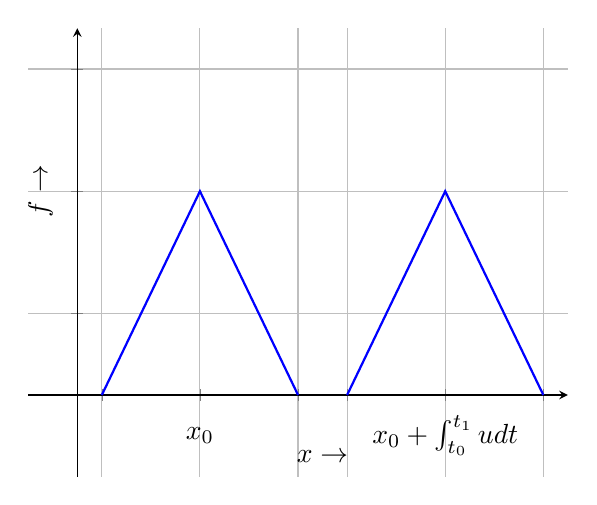
\begin{tikzpicture}
		\begin{axis}[
				% xlabel={$x$},
				% ylabel={$f(x)$},
				axis lines=middle,
				grid=both,
				xmax=10,
				xmin=-1,
				ymax=4.5,
				ymin=-1,
				domain=2:10,
				samples=100,
				xtick={0.5,2.5,4.5, 5.5, 7.5, 9.5},
				ytick={1, 2.5, 4},
				xticklabel=\empty,
				yticklabel=\empty,
			]
			\node at (axis cs:5,-0.75) {$x \rightarrow$};
			\node at (axis cs:-0.75,2.5) [rotate=90] {$f \rightarrow$};
			\draw[thick, blue] (0.5,0) -- (2.5,2.5) -- (4.5,0);
			\draw[thick, blue] (5.5,0) -- (7.5,2.5) -- (9.5,0);
			\node at (axis cs:2.5,-0.5) {$x_0$};
			\node at (axis cs:7.5,-0.5) {$x_0 + \int^{t_1}_{t_0}udt$};
		\end{axis}
	\end{tikzpicture}
	\caption{Triangular property distribution}
	\label{fig:triangularprop}
\end{figure}

\begin{enumerate}[noitemsep]
	\item \textbf{Hyperbolic:} 1$^{st}$ order partial equation $\rightarrow$ 1 family of characteristic equation in real domain.
	\item \textbf{Hyperbolic:} 2$^{nd}$ order partial equation $\rightarrow$ 2 distinct and real set of characteristic equations.
	\item \textbf{Parabolic:} 2$^{nd}$ order partial equation $\rightarrow$ 2 equal and real set of characteristic equations.
	\item \textbf{Elliptical:} 2$^{nd}$ order partial equation $\rightarrow$ 2 distinct and complex set of characteristic equations.
\end{enumerate}

\begin{align*}
	\frac{\partial f}{\partial t} + u \frac{\partial f}{\partial x} = 0 \;
	 & \begin{cases}
		   u = \text{constant} & \Rightarrow \text{linear PDE },     \\
		   u = u(x,t)          & \Rightarrow \text{linear PDE },     \\
		   u = u(x,t,f)        & \Rightarrow \text{quasi-linear PDE}
	   \end{cases}
\end{align*}

\begin{align*}
	a(x,t,f)\frac{\partial f}{\partial t} + b(x,t,f)\frac{\partial f}{\partial x} = 0 \tag{6.5} \label{eq:quasi-linear-ab}
\end{align*}

Above \myeqref{eq:quasi-linear-ab} is quasi-linear PDE, having characteristic equation in real domain $\Rightarrow \frac{dx}{dt} = \frac{b}{a}$

\begin{align*}
	a(x,t,f)\frac{\partial f}{\partial t} + b(x,t,f)\frac{\partial f}{\partial x} = c(x,t,f) \tag{6.6} \label{eq:semi-linear-abc}
\end{align*}

Above \myeqref{eq:semi-linear-abc} is semi-linear PDE, having characteristic equation in real domain.

\clearpage

\section{Lecture 7 22/01/2025}
General quasi-linear 2$^{nd}$ order PDE:
\begin{align*}
	A\frac{\partial^2 f}{\partial x^2} + B\frac{\partial^2 f}{\partial x \partial y} + C\frac{\partial^2 f}{\partial y^2} + D\frac{\partial f}{\partial x} + E\frac{\partial f}{\partial y} + Ff = G \tag{7.1} \label{eq:genral-quasi-linear-pde}
\end{align*}

i.e. $A,B,C$ can be function of $x,y,f,\frac{\partial f}{\partial x}$ and $\frac{\partial f}{\partial y}$.

To find sign of dicriminant $B^2 - 4AC$ tells the classification of equation:
\begin{align*}
	B^2 - 4AC
	\begin{cases}
		> 0, & \text{ Hyperbolic PDE} \\
		= 0, & \text{ Parabolic PDE}  \\
		< 0, & \text{ Elliptical PDE}
	\end{cases}
\end{align*}

This is analogus to general equation of conic-section curves. Which is general by \myeqref{eq:genral-conic-section}
\begin{align*}
	Ay^2 + Bxy + Cx^2 + Dx + Ey + F = 0 \tag{7.2} \label{eq:genral-conic-section}
\end{align*}
\begin{align*}
	B^2 - 4AC
	\begin{cases}
		> 0, & \text{ Hyperbola} \\
		= 0, & \text{ Parabola}  \\
		< 0, & \text{ Ellipse}
	\end{cases}
\end{align*}

\begin{align*}
	df                                       & = \frac{\partial f}{\partial x}dx + \frac{\partial f}{\partial y}dy \tag{7.3} \label{eq:df}                     \\
	d\Big(\frac{\partial f}{\partial x}\Big) & = \frac{\partial^2 f}{\partial x^2}dx + \frac{\partial^2 f}{\partial x \partial y}dy \tag{7.4} \label{eq:dpfpx} \\
	d\Big(\frac{\partial f}{\partial y}\Big) & = \frac{\partial^2 f}{\partial x \partial y}dx + \frac{\partial^2 f}{\partial y^2}dy \tag{7.5} \label{eq:dpfpy}
\end{align*}

Unknown in \myeqref{eq:df}, \myeqref{eq:dpfpx} and \myeqref{eq:dpfpy} are 2$^{nd}$ order derivatives.

From \myeqref{eq:genral-quasi-linear-pde},
\begin{align*}
	A\frac{\partial^2 f}{\partial x^2} + B\frac{\partial^2 f}{\partial x \partial y} + C\frac{\partial^2 f}{\partial y^2} & = - D\frac{\partial f}{\partial x} - E\frac{\partial f}{\partial y} - Ff + G \tag{7.6} \label{eq:genral-quasi-linear-pde-reodered}
\end{align*}

From \myeqref{eq:dpfpx},
\begin{align*}
	\frac{\partial^2 f}{\partial x^2}dx + \frac{\partial^2 f}{\partial x \partial y}dy & = d\Big(\frac{\partial f}{\partial x}\Big) \tag{7.7} \label{eq:dpfpx-reodered}
\end{align*}

From \myeqref{eq:dpfpy},
\begin{align*}
	\frac{\partial^2 f}{\partial x \partial y}dx + \frac{\partial^2 f}{\partial y^2}dy & = d\Big(\frac{\partial f}{\partial y}\Big) \tag{7.8} \label{eq:dpfpy-reordered}
\end{align*}

Matrix representation of \myeqref{eq:genral-quasi-linear-pde-reodered}, \myeqref{eq:dpfpx-reodered} and \myeqref{eq:dpfpy-reordered}:
\begin{align*}
	\underbrace{
		\begin{bmatrix}
			A  & B  & C  \\
			dx & dy & 0  \\
			0  & dx & dy
		\end{bmatrix}
	}_{\text{det(\textbf{A}) = 0}}
	\begin{bmatrix}
		\frac{\partial^2 f}{\partial x^2}          \\
		\frac{\partial^2 f}{\partial x \partial y} \\
		\frac{\partial^2 f}{\partial y^2}
	\end{bmatrix}
	=
	\begin{bmatrix}
		-D\frac{\partial f}{\partial x} - E\frac{\partial f}{\partial y} - Ff + G \\
		d\Big(\frac{\partial f}{\partial x}\Big)                                  \\
		d\Big(\frac{\partial f}{\partial y}\Big)
	\end{bmatrix}.
\end{align*}

Determintant of $(\textbf{A})$ should be equal to zero, i.e.,
\begin{align*}
	\text{det}(\textbf{A})                                    & = 0                                      \\
	A(dy)^2 - B(dxdy) + C(dx)^2                               & = 0                                      \\
	A\Big(\frac{dy}{dx}\Big)^2 - B\Big(\frac{dy}{dx}\Big) + C & = 0 \tag{7.9} \label{eq:matrix-form-pde}
\end{align*}

Solution of above \myeqref{eq:matrix-form-pde} are 2 characteristic equations:
\begin{align*}
	\frac{dy}{dx} & = \frac{B \pm \sqrt{B^2 - 4AC}}{2A}
\end{align*}

\begin{align*}
	\text{if } B^2-4AC > 0 \Rightarrow & \text{2 distinct Real roots}                 \\
	                                   & \text{Family of char. curve}\in \mathbb{R}   \\
	                                   & \text{Hyperbolic PDE}                        \\
	\text{if } B^2-4AC = 0 \Rightarrow & \text{Real and equal roots}                  \\
	                                   & \text{1 Family of char. curve}\in \mathbb{R} \\
	                                   & \text{Parabolic PDE}                         \\
	\text{if } B^2-4AC < 0 \Rightarrow & \text{Imaginary roots}                       \\
	                                   & \text{Family of char. curves}\in \mathbb{C}  \\
	                                   & \text{Elliptic PDE}
\end{align*}

Examples:
\yellownote{
	Incomplete \\
}

\clearpage

\section{Lecture 08/01/2025}
\subsection{Heat Equation}
\begin{align*}
	k\frac{\partial^2 T}{\partial x^2} - \frac{\partial T}{\partial t} = 0 \tag{8.1} \label{eq:2ndorderquasilinearpde}
\end{align*}

\myeqref{eq:2ndorderquasilinearpde} can be decomposed into pair of PDEs:
\begin{align*}
	\frac{\partial^2 T}{\partial x \partial t}dx + \frac{\partial^2 T}{\partial t^2}dt &= d\Big(\frac{\partial T}{\partial t}\Big) \tag{8.2} \label{eq:8.2} \\
	\frac{\partial^2 T}{\partial x^2}dx + \frac{\partial^2 T}{\partial x \partial t}dt &= d\Big(\frac{\partial T}{\partial x}\Big) \tag{8.3} \label{eq:8.3}
\end{align*}

Rewriting \myeqref{eq:2ndorderquasilinearpde}, \myeqref{eq:8.2} and \myeqref{eq:8.3} into matrix form:
\begin{align*}
	\underbrace{
		\begin{bmatrix}
			k  & 0  & 0  \\
			0  & dx & dt \\
			dx & dt & 0
		\end{bmatrix}}_{\text{A}}
	\begin{bmatrix}
		\frac{\partial^2 T}{\partial x^2}          \\
		\frac{\partial^2 T}{\partial x \partial t} \\
		\frac{\partial^2 T}{\partial t^2}
	\end{bmatrix}
	= \begin{bmatrix}
		  \frac{\partial T}{\partial t}            \\
		  d\left(\frac{\partial T}{\partial t}\right) \\
		  d\left(\frac{\partial T}{\partial x}\right)
	  \end{bmatrix}
\end{align*}

\begin{align*}
	\text{det (A)}                        & = 0 \\
	k(0-(dt)^2) - 0(0-dxdt) + 0(0-(dx)^2) & = 0 \\
	-k(dt)^2                              & = 0
\end{align*}

\begin{align*}
	\therefore dt & = 0             \\
	t             & = \text{const.}
\end{align*}

Therefore the equation represents Parabolic PDE (2$^{\text{n}}$ order quasi-linear PDE).

\subsection{1-D Wave Equation}

\begin{align*}
	\frac{\partial^2 f}{\partial t^2}                                                                                                                     & = c^2\frac{\partial^2 f}{\partial x^2} \tag{8.4} \label{eq:1dwaveequation} \\
	\underbrace{\Big(\frac{\partial^2}{\partial t^2} - c^2\frac{\partial^2}{\partial x^2}\Big)}_{\text{Operator acting on f}}f                            & = 0                                                                        \\
	\Big[\Big(\frac{\partial}{\partial t} - c\frac{\partial}{\partial x}\Big) \Big(\frac{\partial}{\partial t} + c\frac{\partial}{\partial x}\Big)\Big] f & = 0 \tag{8.5} \label{eq:char-eq}
\end{align*}

Above \myeqref{eq:char-eq} is pair two 1-D advection equations with constant speed \textit{c} in \textbf{negative} x-direction and \textbf{positive} x-direction respectively.

Discrimant of \myeqref{eq:1dwaveequation}, for A = 1, B=0, C=-1:
\begin{align*}
	B^2 - 4AC      &    \\
	0^2 - 4c^2(-1) &    \\
	4c^2           & >0
\end{align*}

Therefore \myeqref{eq:1dwaveequation} represents Hyperbolic PDE.

\begin{figure}[ht!]
	\centering
	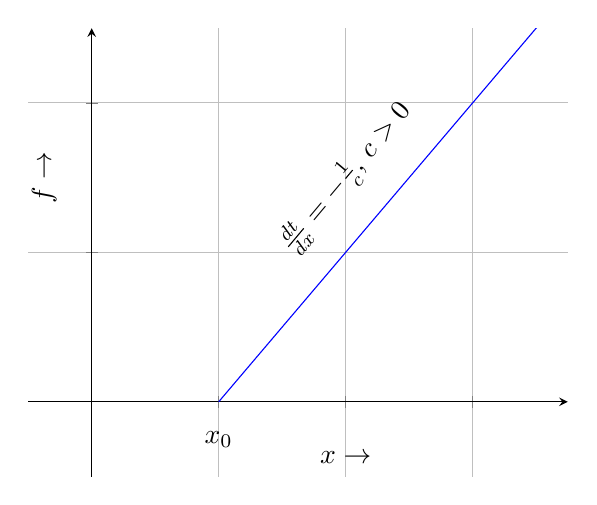
\begin{tikzpicture}
		\begin{axis}[
				% xlabel={$x$},
				% ylabel={$f(x)$},
				axis lines=middle,
				grid=both,
				xmax=7.5,
				xmin=-1,
				ymax=5,
				ymin=-1,
				domain=2:8,
				samples=100,
				xtick={2,4,6,8},
				ytick={2,4},
				xticklabel=\empty,
				yticklabel=\empty,
			]
			\addplot[blue] {-2 + 1*x};
			\node at (axis cs:2,-0.5) {$x_0$};
			\node at (axis cs:4,-0.75) {$x \rightarrow$};
			\node at (axis cs:-0.75,3) [rotate=90] {$f \rightarrow$};
			\node at (axis cs:4,3) [rotate=50] {$\frac{dt}{dx}=-\frac{1}{c}$, $c>0$};
		\end{axis}
	\end{tikzpicture}
	% \label{fig:pathline}
\end{figure}

\begin{figure}[ht!]
	\centering
	\begin{tikzpicture}
		\begin{axis}[
				% xlabel={$x$},
				% ylabel={$f(x)$},
				axis lines=middle,
				grid=both,
				xmax=7.5,
				xmin=-1,
				ymax=5,
				ymin=-1,
				domain=2:6,
				samples=100,
				xtick={2,4,6},
				ytick={2,4},
				xticklabel=\empty,
				yticklabel=\empty,
			]
			\addplot[blue] {6 - 1*x};
			\node at (axis cs:6,-0.5) {$x_0$};
			\node at (axis cs:4,-0.75) {$x \rightarrow$};
			\node at (axis cs:-0.75,3) [rotate=90] {$f \rightarrow$};
			\node at (axis cs:4,3) [rotate=-50] {$\frac{dt}{dx}=-\frac{1}{c}$, $c<0$};
		\end{axis}
	\end{tikzpicture}
	% \label{fig:pathline}
\end{figure}


\begin{align*}
	\frac{\partial^2 f}{\partial x \partial t}dx + \frac{\partial^2 f}{\partial t^2}dt = d\Big(\frac{\partial f}{\partial t}\Big) \tag{8.5} \label{eq:8.5} \\
	\frac{\partial^2 f}{\partial x^2}dx + \frac{\partial^2 f}{\partial x \partial t}dt = d\Big(\frac{\partial f}{\partial x}\Big) \tag{8.6} \label{eq:8.6}
\end{align*}

Rewriting \myeqref{eq:1dwaveequation}, \myeqref{eq:8.5} and \myeqref{eq:8.6} into matrix form:
\begin{align*}
	\underbrace{
		\begin{bmatrix}
			c^2 & 0  & -1 \\
			0   & dx & dt \\
			dx  & dt & 0
		\end{bmatrix}}_{\text{A}}
	\begin{bmatrix}
		\frac{\partial^2 f}{\partial x^2}          \\
		\frac{\partial^2 f}{\partial x \partial t} \\
		\frac{\partial^2 f}{\partial t^2}
	\end{bmatrix}
	= \begin{bmatrix}
		  \frac{\partial f}{\partial t}            \\
		  d\Big(\frac{\partial f}{\partial t}\Big) \\
		  d\Big(\frac{\partial f}{\partial x}\Big)
	  \end{bmatrix}
\end{align*}

\begin{align*}
	\text{det (A)}                             & = 0 \\
	c^2(0-(dt)^2) - 0(0-dxdt) + (-1)(0-(dx)^2) & = 0 \\
	-c^2(dt)^2 + (dx)^2                        & = 0 \\
	-c^2\Big(\frac{dt}{dx}\Big)^2 + 1          & = 0 \\
	c^2\Big(\frac{dt}{dx}\Big)^2 - 1           & = 0
\end{align*}

Slope $\frac{dt}{dx}$ is equal to:
\begin{align*}
	\frac{dt}{dx} & = \frac{-0 \pm \sqrt{0^2 -4 \cdot c^2\cdot (-1)}}{2\cdot c^2} \\
	\frac{dt}{dx} & = \pm \frac{1}{2c}
\end{align*}

\subsection{Laplace Equation}
\begin{align*}
	\frac{\partial^2 f}{\partial x^2} + \frac{\partial^2 f}{\partial y^2}           &= 0 \tag{8.7} \label{eq:8.7}
\end{align*}


\begin{align*}
	\frac{\partial^2 f}{\partial x \partial y}dx + \frac{\partial^2 f}{\partial y^2}dy &= d\left(\frac{\partial f}{\partial y}\right) \tag{8.8} \label{eq:8.8} \\
	\frac{\partial^2 f}{\partial x^2}dx + \frac{\partial^2 f}{\partial x \partial y}dy &= d\left(\frac{\partial f}{\partial x}\right) \tag{8.9} \label{eq:8.0}
\end{align*}

Discrimant of \myeqref{eq:8.7}, for A = 1, B=0, C=1:
\begin{align*}
	B^2 - 4AC     &    \\
	0^2 - 4(1)(1) &    \\
	-4            & <0
\end{align*}

Therefore \myeqref{eq:8.7} represents Elliptical PDE.

Rewriting \myeqref{eq:8.7}, \myeqref{eq:8.8} and \myeqref{eq:8.9} into matrix form:
\begin{align*}
	\underbrace{
		\begin{bmatrix}
			1 & 0  & 1 \\
			0   & dx & dy \\
			dx  & dy & 0
		\end{bmatrix}}_{\text{A}}
	\begin{bmatrix}
		\frac{\partial^2 f}{\partial x^2}          \\
		\frac{\partial^2 f}{\partial x \partial y} \\
		\frac{\partial^2 f}{\partial y^2}
	\end{bmatrix}
	= \begin{bmatrix}
		  0                                        \\
		  d\left(\frac{\partial f}{\partial y}\right) \\
		  d\left(\frac{\partial f}{\partial x}\right)
	  \end{bmatrix}
\end{align*}

\begin{align*}
	\text{det (A)}                        & = 0 \\
	1(0-(dy)^2) - 0(0-dxdy) + 1(0-(dx)^2) & = 0 \\
	-(dy)^2 - (dx)^2                      & = 0 \\
	\left(\frac{dy}{dx}\right)^2 + 1         & = 0 \\
	\frac{dy}{dx}                         & = \pm \iota
\end{align*}

\clearpage

\section{Lecture 9 28/01/2025}
\begin{itemize}
	\item Domain of dependence at a given point in the solution domain would corresponding to the region where solution will impact solution will be impacted by the solution at the above given point.
	\item Range of independence at a given point in the solution domain would corresponding to the region where solution will impact solution will be impacted by the solution at the above given point.
\end{itemize}

\subsection{Wave Equation}
Hyperbolic PDE:
\begin{align*}
	\frac{\partial^2 f}{\partial t^2} &= c^2\frac{\partial^2 f}{\partial x^2} \tag{9.1} \label{eq:9.1}
\end{align*}

Parabolic PDE:
\begin{align*}
	\frac{\partial T}{\partial t} &= c^2\frac{\partial T}{\partial x} \tag{9.2} \label{eq:9.2}
\end{align*}

Ellipse PDE:
\begin{align*}
	\frac{\partial^2 f}{\partial t^2} + \frac{\partial^2 f}{\partial x^2} &= 0 \tag{9.3} \label{eq:9.3}
\end{align*}

\yellownote{Add figs}

\begin{align*}
	a\frac{\partial f}{\partial x} + b\frac{\partial f}{\partial x} + c\frac{\partial g}{\partial t} + d\frac{\partial g}{\partial x} &= e \tag{9.4} \label{eq:9.4}\\
	A\frac{\partial f}{\partial x} + B\frac{\partial f}{\partial x} + C\frac{\partial g}{\partial t} + D\frac{\partial g}{\partial x} &= E \tag{9.5} \label{eq:9.5}
\end{align*}

Using chain rule;
\begin{align*}
        \frac{\partial f}{\partial t}dt + \frac{\partial f}{\partial x}dx &= df \tag{9.6} \label{eq:9.6}\\
        \frac{\partial g}{\partial t}dt + \frac{\partial g}{\partial x}dx  &= dg \tag{9.7} \label{eq:9.7}
\end{align*}

Rewriting \myeqref{eq:9.4}, \myeqref{eq:9.5}, \myeqref{eq:9.6} and \myeqref{eq:9.7} into matrix form:
\begin{align*}
	\underbrace{
		\begin{bmatrix}
			a  & b & c & d \\
			A  & B & C & D \\
			dt & dx & 0 & 0\\
			0  & 0 & dt & dy
		\end{bmatrix}}_{\text{A}}
	\begin{bmatrix}
		\frac{\partial f}{\partial t} \\
		\frac{\partial f}{\partial x} \\
		\frac{\partial g}{\partial t} \\
		\frac{\partial g}{\partial x}
	\end{bmatrix}
	= \begin{bmatrix}
		e \\
		E \\
		df \\
		dg
	  \end{bmatrix}
\end{align*}

\begin{align*}
	\text{det (A)}                        & = 0 \\
	(dx)^2\underbrace{(aC-Ac)}_{\overline{A}} - (dx)(dt)\underbrace{(aD-Ad+bC-Bc)}_{\overline{B}} & \\ + (dt)^2\underbrace{(bD-Bd)}_{\overline{C}} & = 0
\end{align*}

Discrimant of \myeqref{eq:8.7}, for $\overline{A}=(aC-Ac)$, $\overline{B}=(aD-Ad+bC-Bc)$, $\overline{C}=(bD-Bd)$:
\begin{align*}
	\overline{B}^2 - 4\overline{A}\overline{C} &  \\
	(aD-Ad+bC-Bc)^2 - 4(aC-Ac)(bD-Bd)
\end{align*}

\begin{align*}
	\frac{dx}{dt} = \frac{\overline{B} \pm \sqrt{\overline{B}^2 - 4\overline{A}\overline{C}}}{2\overline{A}} \tag{9.8} \label{eq:9.8}
\end{align*}

Depending upon sign of $\overline{B}^2 - 4\overline{A}\overline{C}$ the follwing classification can be made:
\begin{itemize}[noitemsep]
	\item Negative $\rightarrow$ Elliptic
	\item Zero $\rightarrow$ Parabolic
	\item positive $\rightarrow$ Hyperbolic
\end{itemize}

\subsection{Heat Transfer Equation}
\begin{align*}
	\frac{\partial T}{\partial t} &= k \frac{\partial^2 T}{\partial x^2} \tag{9.9} \label{eq:9.9}
\end{align*}
where, $k$ is coeffeicent of thermal expansion.

\yellownote{Figure}

Applying FTCS (Forward Time and Central in Space) scheme,
\begin{align*}
	t_n &= n\Delta t &, n&=0,1,2,\dots \\
	x_m &= x_0 + m\Delta x &, m&=0,1,2,\dots, N
\end{align*}

Backward difference:
\begin{align*}
	\left(\frac{\partial T}{\partial t}\right)_{x,t} &= \frac{T_{m,n+1} - T_{m,n}}{\Delta t}  \tag{9.10} \label{eq:9.10}
\end{align*}

Central difference:
\begin{align*}
	\left(\frac{\partial^2 T}{\partial t^2}\right)_{x,t} &= \frac{T_{m+1,n} - 2\cdot T_{m,n} + T_{m-1,n}}{\Delta t} \tag{9.11} \label{eq:9.11}
\end{align*}

Substituting \myeqref{eq:9.10} and \myeqref{eq:9.11} into \myeqref{eq:9.9}, we obtain,
\begin{align*}
	\left(\frac{T_{m,n+1} - T_{m,n}}{\Delta t}\right) &= k\left(\frac{T_{m+1,n} - 2\cdot T_{m,n} + T_{m-1,n}}{\Delta t}\right) \\
	T_{m,n+1} = T_{m,n} &+ \underbrace{\frac{k\Delta t}{(\Delta x)^2}}_{\lambda}\left(T_{m+1,n} - 2T_{m,n} + T_{m-1,n}\right) \\
	T_{m,n+1} = &(1-2\lambda)T_{m,n} + \lambda T_{m-1,n} + \lambda T_{m+1,n}
\end{align*}

\yellownote{Incomplete}

\clearpage

\section{Lecture 10 29/01/2025}
\subsection{Lax Theorem}
The \textbf{Lax Equivalence Theorem} is a fundamental result in numerical analysis that provides a necessary and sufficient condition for the convergence of finite difference schemes used to approximate solutions of partial differential equations (PDEs).

For a well-posed initial value problem, a consistent finite difference scheme is convergent if and only if it is stable.

Key Concepts: \begin{itemize}[noitemsep]
    \item \textbf{Consistency:} A finite difference scheme is said to be \textit{consistent} if the truncation error tends to zero as the grid spacing (\(\Delta x, \Delta t\)) approaches zero.
    \item \textbf{Stability:} A scheme is \textit{stable} if numerical errors do not grow uncontrollably as time progresses.
    \item \textbf{Convergence:} A numerical scheme is \textit{convergent} if the solution obtained from the scheme approaches the exact solution as the grid is refined.
\end{itemize}

Let \( u(x,t) \) be the exact solution of a PDE, and let \( u^n_j \) be the numerical solution at time level \( n \) and spatial index \( j \). The numerical scheme can be written as:
\begin{align*}
    u^{n+1}_j = F(u^n_{j-1}, u^n_j, u^n_{j+1}, \dots),
\end{align*}
where \( F \) is the finite difference operator.

For the scheme to be \textbf{consistent}, the local truncation error must satisfy:
\begin{align*}
    \lim_{\Delta x, \Delta t \to 0} \text{(Truncation Error)} = 0.
\end{align*}

\textbf{By Lax's theorem}, if the scheme is consistent and stable, it is guaranteed to be convergent:
\begin{align*}
    \lim_{\Delta x, \Delta t \to 0} || u^n_j - u(x_j, t_n) || = 0.
\end{align*}

Significance of Lax’s theorem is that it provides a crucial guideline for designing numerical methods:
\begin{itemize}[noitemsep]
    \item Ensuring \textbf{consistency} is relatively straightforward by comparing the difference scheme with the PDE.
    \item \textbf{Stability} is often more challenging and requires analysis techniques like Von Neumann stability analysis.
    \item If a scheme is both \textbf{consistent and stable}, it is guaranteed to be \textbf{convergent}, meaning it will correctly approximate the true solution.
\end{itemize}

\subsection{Van Neumann}
Van Neumann stability analysis is a mathematical technique used to assess the stability of finite difference schemes for solving partial differential equations (PDEs). It is particularly useful in analyzing the behavior of numerical solutions over time.

Key Idea: The method is based on applying a Fourier mode decomposition to the numerical scheme. The numerical solution is expressed as a sum of Fourier modes, and the growth factor 

Stability Criterion: A finite difference scheme is \textbf{stable} if and only if the magnitude of the amplification factor satisfies \myeqref{eq:vanneumann}:
\begin{align*}
	|G(k)| \leq 1, \quad \forall k. \tag{10.1} \label{eq:vanneumann}
\end{align*}
This ensures that numerical errors do not grow uncontrollably as time progresses.

\begin{enumerate}[noitemsep]
    \item \textbf{Express the numerical scheme} as a recurrence relation.
    \item \textbf{Substitute a Fourier mode} of the form:
    \begin{align*}
        u^n_j = \hat{u}^n e^{i k j \Delta x},
    \end{align*}
    where \( i \) is the imaginary unit, \( k \) is the wave number, and \( \Delta x \) is the spatial step size.
    \item \textbf{Determine the amplification factor} \( G(k) \) by solving for:
    \begin{align*}
        G(k) = \frac{\hat{u}^{n+1}}{\hat{u}^n}.
    \end{align*}
    \item \textbf{Check the stability condition} \( |G(k)| \leq 1 \).
\end{enumerate}

Application : Van Neumann analysis is commonly used for schemes solving hyperbolic PDEs, such as the \textbf{heat equation}, \textbf{wave equation}, and \textbf{advection equation}. It helps determine whether a numerical method will produce bounded solutions over time.

For \textbf{stability}, we often use techniques like the \textbf{Von Neumann stability analysis} to check that perturbations do not grow indefinitely using \myeqref{eq:vanneumann}.

\clearpage
\section{Lecture 11 03/02/2025}
\subsection{Van Neumann Stability Analysis For 1-D Heat Conducting Equation For FTCS Scheme}
\begin{align*}
	\frac{\partial T}{\partial t} &= k\frac{\partial^2 T}{\partial x^2} \tag{11.1} \label{eq:1dheateq}
\end{align*}

Appling FTCS scheme:
\begin{align*}
	\frac{T_{m,n+1} - T_{m,n}}{\Delta t} &= k\left[\frac{T_{m+1,n}-2T_{m,n}+T_{m-1,n}}{(\Delta x)^2}\right] \tag{11.2} \label{eq:1dheatftcseq}
\end{align*}

Let $\lambda = k \Delta t / (\Delta x)^2$

Since error $\epsilon_{m,n}$ identically satisfies difference equations, we can write;
\begin{align*}
	\epsilon{m,n+1} &= \epsilon_{m,n} + \lambda \left(\epsilon_{m+1,n} + \epsilon_{m-1,n} -2 \epsilon_{m,n}\right) \\
	\epsilon{m,n+1} &= \left(1-2\lambda \right)\epsilon_{m,n} + \lambda \left(\epsilon_{m+1,n} + \epsilon_{m-1,n} \right) \tag{11.3} \label{eq:11.3}
\end{align*}

Let $\epsilon_{m,n} = \exp(at) \cdot \exp(ikx)$

Since, $t = n \Delta t$ and $x = m \Delta x$; 
\begin{align*}
	\epsilon_{m,n} &= \exp(an \Delta t) \cdot \exp(ik m \Delta x) \tag{11.4} \label{eq:11.4}
\end{align*}

Substituting \myeqref{eq:11.4} in \myeqref{eq:11.3}, we obtain;
\begin{align*}
	 & e^{(a(n+1)\Delta t)} \cdot e^{(ik m \Delta x)} = (1-2\lambda)e^{(an\Delta t)}e^{(ik m \Delta x)} \\ &+ \lambda\left[e^{(ik (m+1) \Delta x)} + e^{(ik (m-1) \Delta x)} \right]e^{(an\Delta t)} \\
	 & e^{(an\Delta t)} \cdot e^{(ik m \Delta x)} = (1-2\lambda)e^{(an\Delta t)}e^{(ik m \Delta x)} \\ &+ \lambda\left[e^{(ik (m+1) \Delta x)} + e^{(ik (m-1) \Delta x)} \right] \tag{11.5} \label{eq:11.5}
\end{align*}

Divide both sides of \myeqref{eq:11.5} by $e^{(ik m \Delta x)}$
\begin{align*}
	e^{(a\Delta t)} &= (1-2\lambda) + \lambda \underbrace{\left[e^{(ik \Delta x)} + e^{-(ik \Delta x)} \right]}_{2\cos(k\Delta x)} \\
	e^{(a\Delta t)} &= (1-2\lambda) + 2\lambda \cos(k\Delta x) \\
	e^{(a\Delta t)} &= 1- 2\lambda\left[1- \cos(k\Delta x)\right] \\
	e^{(a\Delta t)} &= 1- 4\lambda\left[\sin^2\left(\frac{k\Delta x}{2}\right)\right] \tag{11.6} \label{eq:11.6}
\end{align*}

Amplification factor
\begin{align*}
	G &= \left|\frac{\epsilon_{m,n+1}}{\epsilon_{m,n}}\right| \\
	  &= \left|\frac{e^{a(n+1)\Delta x} \cdot e^{ikm\Delta x}}{e^{an\Delta x} \cdot e^{ikm\Delta x}}\right| \\
	  &= \left|e^{a\Delta x}\right| \tag{11.7} \label{eq:11.7}
\end{align*}

FTCS scheme will be stable if
\begin{align*}
	\left|e^{a\Delta t}\right| \leq 1 \Rightarrow \left|1 - 4\lambda\left[\sin^2\left(\frac{k\Delta x}{2}\right)\right] \right| \leq 1
\end{align*}

The following 2 conditions has to be identically satisfied
\begin{align*}
	1 - 4\lambda\left[\sin^2\left(\frac{k\Delta x}{2}\right)\right] &\leq 1 \tag{11.8.i} \label{eq:11.8.i} \\
	1 - 4\lambda\left[\sin^2\left(\frac{k\Delta x}{2}\right)\right] &\geq -1 \tag{11.8.ii} \label{eq:11.8.ii}
\end{align*}

For \myeqref{eq:11.8.i};
\begin{align*}
	1 - 4\lambda\left[\sin^2\left(\frac{k\Delta x}{2}\right)\right] &\leq 1 \\
	- 4\lambda\left[\sin^2\left(\frac{k\Delta x}{2}\right)\right] &\leq 0
\end{align*}
Therefore, it is always true.

For \myeqref{eq:11.8.ii};
\begin{align*}
	1 - 4\lambda\left[\sin^2\left(\frac{k\Delta x}{2}\right)\right] &\geq 1 \\
	4\lambda\left[\sin^2\left(\frac{k\Delta x}{2}\right)\right] &\leq 2
\end{align*}
Maximum magnitude of $\sin^2\left(k\Delta x/2\right)=1$
\begin{align*}
	4\lambda \cdot 1 &\leq 2 \\
	\lambda &\leq \frac{1}{2} \\
	\frac{k\Delta t}{(\Delta x)} &\leq \frac{1}{2} \\
	\Delta t &\leq \frac{(\Delta x)^2}{2k}
\end{align*}

\clearpage

\section{Lecture 12 04/02/2025}
\subsection{BTCS Scheme}
\begin{align*}
	\frac{\partial T}{\partial t} &= k\frac{\partial^2 T}{\partial x^2} \tag{12.1} \label{eq:1dheateq1} \\
	\frac{T_{m,n} - T_{m,n-1}}{\Delta t} &= k\left[\frac{T_{m+1,n} - 2\cdot T_{m,n} + T_{m-1,n}}{(\Delta x)^2}\right] \tag{12.2} \label{eq:btcs}
\end{align*}

Let $\lambda = k\Delta t/(\Delta x)^2$
\begin{align*}
	(1+2\lambda)T_{m,n} - \lambda(T_{m+1,n} + T_{m-1,n}) &= T_{m,n-1} \tag{12.3} \label{12.3}
\end{align*}

For stability;
\begin{align*}
	(1+2\lambda)\epsilon_{m,n} &- \lambda(\epsilon_{m+1,n} + \epsilon_{m-1,n}) = \epsilon_{m,n-1} \tag{12.4} \label{eq:12.4}\\
	\epsilon_{m,n} &= B^{\mu n\Delta t}\exp(ikm\Delta x) \tag{12.5} \label{eq:12.5}
\end{align*}

Substituting \myeqref{eq:12.5} in \myeqref{eq:12.4}, we obtain;
\begin{align*}
	\begin{rcases}
		&(1 + 2\lambda)B^{\mu n \Delta t} e^{(ikm\Delta x)} \\ &-\lambda B^{\mu n \Delta t} \left(e^{(ik(m+1)\Delta x)} + e^{(ik(m-1)\Delta x)}\right) \\ &= B^{\mu (n-1)\Delta t}e^{ikm\Delta x}
	\end{rcases} & \tag{12.6} \label{eq:12.6}
\end{align*}

Divide \myeqref{eq:12.6} throughout by $B^{\mu (n-1) \Delta t}\cdot e^{(ikm\Delta x)}$
\begin{align*}
	(1 + 2\lambda)B^{\mu \Delta t} - \lambda B^{\mu \Delta t} \left(e^{(ik\Delta x)} + e^{-(ik\Delta x)}\right) &=1 \\
	(1 + 2\lambda)B^{\mu \Delta t} - 2\lambda B^{\mu \Delta t} \cos(k\Delta x)&=1 \\
	B^{\mu \Delta t} \left(1 + 2\lambda - 2\lambda\cos(k\Delta x)\right) &=1 \\
	B^{\mu \Delta t} \left(1 + 2\lambda[1 - \cos(k\Delta x)]\right) &=1 \\
	B^{\mu \Delta t} \left(1 + 4\lambda\sin^2\left(\frac{k\Delta x}{2}\right)\right)&=1 \\
	B^{\mu \Delta t} = \frac{1}{\left(1 + 4\lambda\sin^2\left(\frac{k\Delta x}{2}\right)\right)} \tag{12.7} \label{eq:12.7}
\end{align*}

Amplification factor
\begin{align*}
	G = \left|\frac{\epsilon_{m,n+1}}{\epsilon_{m,n}}\right| = \left|B^{\mu \Delta t}\right| \leq 1 \tag{12.8} \label{eq:12.8}
\end{align*}

\myeqref{eq:12.8} shows that BTCS scheme is unconditionally stable.

\subsection{CTCS Scheme / Richardson Scheme}
\begin{align*}
	\frac{T_{m,n+1} - T_{m,n-1}}{2\cdot\Delta t} &= k\left[\frac{T_{m+1,n} - 2\cdot T_{m,n} + T_{m-1,n}}{(\Delta x)^2}\right] \tag{12.9} \label{eq:ctcs}
\end{align*}

Let $\lambda = 2\cdot k\Delta t/(\Delta x)^2$
\begin{align*}
	T_{m,n+1} &= T_{m,n-1} + \lambda(T_{m+1,n} - 2\cdot T_{m,n} + T_{m-1,n}) \tag{12.10} \label{12.10}
\end{align*}

For stability;
\begin{align*}
	\epsilon_{m,n+1} &= \epsilon_{m,n-1} + \lambda(\epsilon_{m+1,n}-2\cdot\epsilon_{m,n} + \epsilon_{m-1,n}) \tag{12.11} \label{eq:12.11} \\
	\epsilon_{m,n} &= B^{\mu n\Delta t}\exp(ikm\Delta x) \tag{12.12} \label{eq:12.12}
\end{align*}

\begin{align*}
	\epsilon_{m,n} &= B^{\mu n\Delta t}e^{(ikm\Delta x)} \\
		       &= B^{\mu (n-1)\Delta t}e^{(ikm\Delta x)} \\ &+ \lambda B^{\mu n \Delta t}\left[e^{ik\Delta x} - e^{-ik\Delta x}\right]e^{ikm\Delta x}
\end{align*}

Divide throughout by $B^{\mu(n-1)\Delta t} e^{ikm\Delta x}$
\begin{align*}
	B^{2\cdot\mu(n-1)\Delta t} = 1 -2\lambda \cdot B^{\mu \Delta t}\left(1-\cos(k\Delta x)\right) \\
	B^{2\cdot\mu(n-1)\Delta t} = 1 -2\lambda \cdot B^{\mu \Delta t}\left(2\cdot\sin^2(k\Delta x)\right) \\
	\left(B^{\mu(n-1)\Delta t}\right)^2 + 4\lambda \cdot \sin^2(k\Delta x)B^{\mu \Delta t} - 1 = 0 \\
	G^2 + \beta G -1 = 0 \tag{12.13} \label{eq:12.13}
\end{align*}

Amplification factor
\begin{align*}
	G &= \left|\frac{\epsilon_{m,n+1}}{\epsilon_{m,n}}\right| = \left|B^{\mu \Delta t}\right| \leq 1 \tag{12.14} \label{eq:12.14} \\
	G_{1,2} &= \frac{-\beta \pm \sqrt{\beta^2 + 4}}{2} \tag{12.15} \label{eq:12.15}
\end{align*}

\myeqref{eq:12.14} shows that CTCS scheme is stable.
\freeyellownote{500}{-320}{To be checked}

\clearpage

\section{Lecture 13 06/02/2025}
\subsection{Crank Nicholson Scheme}
\begin{align*}
	\left(\frac{\partial T}{\partial t}\right)_{m,n+1/2} &= \tilde{k}\left(\frac{\partial^2 T}{\partial x^2}\right)_{m,n+1/2} \tag{13.1} \label{eq:13.1}
\end{align*}
\begin{align*}
	&\frac{T_{m,n} - T_{m,n-1}}{\Delta t} \\ &\quad  \; = \tilde{k}\left[\frac{T_{m+1,n+1/2} - 2T_{m,n+1/2} + T_{m-1,n+1/2}}{(\Delta x)^2}\right] \tag{13.2} \label{eq:13.2}
\end{align*}

Let $\lambda = \tilde{k}\Delta t/2(\Delta x)^2$
\begin{align*}
	(1 + &2\lambda)T_{m,n+1} - \lambda T_{m,n-1} - \lambda T_{m+1,n+1} = \\ &(1 - 2\lambda)T_{m,n} - \lambda T_{m,n} \tag{13.3} \label{eq:13.3}
\end{align*}

For stability;
\begin{align*}
	(1 + &2\lambda)\epsilon_{m,n+1} - \lambda \epsilon_{m+1,n+1} - \lambda \epsilon_{m-1,n+1} = \\ &(1 - 2\lambda)\epsilon_{m,n} - \lambda \epsilon_{m+1,n} + \lambda \epsilon_{m-1,n} \tag{13.4} \label{eq:13.4} \\
	\epsilon_{m,n} &= B^{\mu n\Delta t}\exp(ikm\Delta x) \tag{13.5} \label{eq:13.5}
\end{align*}

Substituting \myeqref{eq:13.4} in \myeqref{eq:13.3}, we obtain;

\begin{align*}
	\begin{rcases}
	&(1 + 2\lambda)B^{\mu (n+1)\Delta t}e^{(ikm\Delta x)} \\ &- \lambda B^{\mu (n+1) \Delta t}\left[e^{ik (m+1) \Delta x} + e^{-ik (m-1) \Delta x}\right] \\ &= (1 - 2\lambda)B^{\mu n\Delta t}e^{ikm\Delta x} \\ &+ \lambda B^{\mu n\Delta t}\left[e^{ik (m+1) \Delta x} + e^{ik (m-1) \Delta x}\right]
	\end{rcases} & \tag{13.6} \label{eq:13.6}
\end{align*}

Divide throughout by $B^{\mu n \Delta t} e^{ikm\Delta x}$
\begin{align*}
	(1 &+ 2\lambda)B^{\mu n\Delta t} - 2\lambda B^{\mu n \Delta t}\left[\cos(k \Delta x)\right] \\ &= (1 - 2\lambda) + 2\lambda \left[\cos(k \Delta x)\right] \\
	(1 &+ 2\lambda - 2\lambda \cos(k \Delta x))B^{\mu n\Delta t} \\ &= (1 - 2\lambda) + 2\lambda \left[\cos(k \Delta x)\right] \\
	(1 &+ 2\lambda(1 - \cos(k \Delta x)))B^{\mu n\Delta t} \\ &= 1 - 2\lambda(1 - \cos(k \Delta x)) \\
	B^{\mu n\Delta t} &= \frac{1 - 2\lambda(1 - \cos(k \Delta x))}{1 + 2\lambda(1 - \cos(k \Delta x))} \\
	B^{\mu n\Delta t} &= \frac{1 - 4\lambda(\sin^2(k \Delta x/2))}{1 + 4\lambda(\sin^2(k \Delta x/2))} \tag{13.7} \label{eq:13.7}
\end{align*}

Let $4\lambda(\sin^2(k \Delta x/2)) = \beta$

Amplification factor
\begin{align*}
	G = \left|\frac{\epsilon_{m,n+1}}{\epsilon_{m,n}}\right| = \frac{1-\beta}{1+ \beta} = \left|B^{\mu \Delta t}\right| \leq 1 \tag{13.8} \label{eq:13.8}
\end{align*}

\subsection{Dufart Frankel Scheme}
\begin{align*}
	\left(\frac{\partial T}{\partial t}\right)_{m,n} &= k\left(\frac{\partial^2 T}{\partial x^2}\right)_{m,n} \tag{13.9} \label{eq:13.9} \\
	\frac{T_{m,n+1} - T_{m,n}}{2\Delta t} &= k\left[\frac{T_{m+1,n} - 2T_{m,n} + T_{m-1,n}}{(\Delta x)^2}\right] \tag{13.10} \label{eq:13.10}
\end{align*}

Let $\lambda = 2 \cdot k\Delta t/(\Delta x)^2$

Taking average $T_{m,n} = \frac{T_{m,n+1} + T_{m,n-1}}{2}$
\begin{align*}
	T_{m,n+1} - T_{m,n} &= \lambda\left[\frac{T_{m+1,n} - 2\left(\frac{T_{m,n+1} + T_{m,n-1}}{2}\right) + T_{m-1,n}}{(\Delta x)^2}\right] \\
	(1+\lambda)T_{m,n+1} &= \lambda T_{m+1,n} + (1 - \lambda)T_{m,n-1} + \lambda T_{m-1,n} \tag{13.11} \label{eq:13.11}
\end{align*}

Errors should satisfy the same difference equation identically;
\begin{align*}
	(1+\lambda)\epsilon_{m,n+1} &= \lambda \epsilon_{m+1,n} + (1 - \lambda)\epsilon_{m,n-1} + \lambda \epsilon_{m-1,n} \tag{13.12} \label{eq:13.12} \\
	\epsilon_{m,n} &= B^{\mu n\Delta t}\exp(ikm\Delta x) \tag{13.13} \label{eq:13.13}
\end{align*}

Substituting \myeqref{eq:13.12} in \myeqref{eq:13.11}, we obtain;
\begin{align*}
	\begin{rcases}
		&(1 +\lambda)B^{\mu (n+1) \Delta t}\exp(ikm\Delta x) \\ &= \lambda B^{\mu n\Delta t}\exp(ik (m+1) \Delta x) \\ &+ (1 - \lambda)B^{\mu (n-1) \Delta t}\exp(ikm \Delta x) \\ &+ \lambda B^{\mu n \Delta t}\exp(ik (m-1) \Delta x)
	\end{rcases} & \tag{13.14} \label{eq:13.14}
\end{align*}

Divide throughout by $B^{\mu n \Delta t} e^{ikm\Delta x}$
\begin{align*}
	(1 +\lambda)\left(B^{\mu \Delta t}\right)^2  &= \lambda B^{\mu \Delta t} \left(2\cos(k\Delta t)\right) + (1-\lambda) \\
	(1 +\lambda)G^2  &= \lambda \left(2\cos(k\Delta t)\right)G + (1 - \lambda) \\
	(1 +\lambda)G^2  &- \lambda \left(2\cos(k\Delta t)\right)G - (1 - \lambda) = 0 \tag{13.15} \label{eq:13.15}
\end{align*}
\begin{align*}
	G_{1,2} &= \frac{2\lambda \cos(k\Delta x) \pm \sqrt{4\lambda^2\cos^2(k\Delta x)+4(1-\lambda^2)}}{2(1+\lambda)} \\
	G_{1,2} &= \frac{\cancel{2}\lambda \cos(k\Delta x) \pm \cancel{2}\sqrt{\lambda^2(\cos^2(k\Delta x) - 1) + 1}}{\cancel{2}(1+\lambda)} \\
	G_{1,2} &= \frac{\lambda \cos(k\Delta x) \pm \sqrt{1 - \lambda^2\sin^2(k\Delta x)}}{(1+\lambda)} \tag{13.16} \label{eq:13.16}
\end{align*}

For Dufart Frankel Scheme to be stable $G_1 \& G_2$ in \myeqref{eq:13.16} should both simultaneously less than 1.

\textbf{Case i}: Quantity under square root is real.

i.e., $1-\lambda^2\sin^2(k\Delta x) \geqslant 0$
\begin{align*}
	G &=  \frac{\lambda \cos(k\Delta x) \pm \sqrt{1 - \lambda^2\sin^2(k\Delta x)}}{(1+\lambda)} \\
	 &\leqslant \frac{\lambda \cos(k\Delta x)+1}{(1+\lambda)} \\
	 &\leqslant \frac{\lambda +1}{(1+\lambda)} \\
	 &\leqslant 1
\end{align*}

\textbf{Case ii}: Quantity under square root is imaginary.

i.e., $1-\lambda^2\sin^2(k\Delta x) \leqslant 0$
\begin{align*}
	G_{1,2} &= \frac{\lambda \cos(k\Delta x) \pm \sqrt{1 - \lambda^2\sin^2(k\Delta x)}}{(1+\lambda)} \\ 
	  &= \frac{\lambda \cos(k\Delta x) \pm \iota \sqrt{\lambda^2\sin^2(k\Delta x) - 1}}{(1+\lambda)} \\
	|G_{1,2}^2| &= \frac{\lambda^2 \cos^2(k\Delta x) + \lambda^2\sin^2(k\Delta x) - 1}{(1+\lambda)^2} \\ 
		    &= \frac{(\lambda^2 - 1)}{(1+\lambda)^2} \\
		    &= \frac{\cancel{(\lambda + 1)}(\lambda - 1)}{(1+\lambda)^{\cancel{2}}} \\
		    &= \frac{(\lambda - 1)}{(1+\lambda)} \\
		    &\leqslant 1
\end{align*}

Therefore Dufart Frankel Scheme is unconditionally stable.

\clearpage

\section{Lecture 14 10/02/2025}
\subsection{2-D Heat Conduction Equation}
\begin{align*}
	\left(\frac{\partial T}{\partial t}\right)_{\smash{m,n,p}} \mspace{-5mu} &= \tilde{k} \left[ \left(\frac{\partial^2 T}{\partial x^2}\right)_{\smash{m,n,p}} \mspace{-5mu} + \left(\frac{\partial^2 T}{\partial y^2}\right)_{\smash{m,n,p}} \right] \tag{14.1} \label{eq:2dheateq}
\end{align*}

Initial conditions: $T(x,y,t=0)$

Boundary conditions: temperatures on 4 sides

\(m \rightarrow l\), \(n \rightarrow y\) and \(p \rightarrow t\)

Applying FTCS:
\begin{align*}
	\begin{rcases}
		\frac{T_{m,n,p+1} - T_{m,n,p}}{\Delta t} \mspace{-15mu} &= \tilde{k}\left[\frac{T_{m+1,n,p} - 2T_{m,n,p} + T_{m-1,n,p}}{(\Delta x)^2}\right] \\ &+ \tilde{k}\left[\frac{T_{m,n+1,p} - 2T_{m,n,p} + T_{m,n-1,p}}{(\Delta y)^2}\right]
	\end{rcases} & \tag{14.2} \label{eq:14.2}
\end{align*}

For stability;
\begin{align*}
	\epsilon_{m,n,p} &= B^{\mu p\Delta t}\exp(ikm\Delta x)\exp(ikn\Delta y) \tag{14.3} \label{eq:14.3} 
\end{align*}

Amplification factor:
\begin{align*}
	G = \left|\frac{\epsilon_{m,n,p+1}}{\epsilon_{m,n,p}}\right| = \left|B^{\mu \Delta t}\right| \leq 1 \tag{14.4} \label{eq:14.4}
\end{align*}

\begin{align*}
	\frac{2k\Delta t}{\left(\Delta x\right)^2} + \frac{2l\Delta t}{\left(\Delta y\right)^2} \leq 1
\end{align*}

if \(\Delta x = \Delta y = d \), \( k = l \)
\begin{align*}
	\frac{4k\Delta t}{\left(\Delta d\right)^2} &\leq 1 \\
	\lambda = \frac{k\Delta t}{\left(\Delta d\right)^2} &\leq \frac{1}{4} \tag{14.5} \label{eq:stabilityconditionfor2dheateq}
\end{align*}

\myeqref{eq:stabilityconditionfor2dheateq} is stability condition for 2-D heat conduction equation.

Apply Crank Nicholson Scheme on 2-D heat conduction equation:
\begin{align*}
	\mspace{-47mu}\left(\frac{\partial T}{\partial t}\right)_{\smash{m,n,p+1/2}} \mspace{-25mu} &= \tilde{k} \left[ \left(\frac{\partial^2 T}{\partial x^2}\right)_{\smash{m,n,p+1/2}} \mspace{-24mu} + \left(\frac{\partial^2 T}{\partial y^2}\right)_{\smash{m,n,p+1/2}} \right] \tag{14.6} \label{eq:14.6}
\end{align*}

\begin{align*}
\mspace{-49mu}
	\begin{rcases}
		\frac{T_{m,n,p+1} - T_{m,n,p}}{\Delta t/2} \mspace{-17mu} &= \tilde{k}\left[\frac{T_{m+1,n,p+1/2} - 2T_{m,n,p+1/2} + T_{m-1,n,p+1/2}}{(\Delta x)^2}\right] \\ & + \tilde{k}\left[\frac{T_{m,n+1,p+1/2} - 2T_{m,n,p+1/2} + T_{m,n-1,p+1/2}}{(\Delta y)^2}\right]
	\end{rcases} & \tag{14.7} \label{eq:14.7}
\end{align*}

Assuming average:
\begin{align*}
	T_{\smash{m,n,p+1/2}} = \left[\frac{T_{\smash{m,n+1,p+1}} + T_{\smash{m+1,n,p-1}}}{2}\right] \tag{14.8} \label{eq:14.8}
\end{align*}

Substituting \myeqref{eq:14.8} in \myeqref{eq:14.6}

ADI method $\rightarrow$ Alternate Directional Implicit method

% \begin{align*}
% \mspace{-49mu}
% 	\begin{rcases}
% 		\frac{T_{m,n,p+1} - T_{m,n,p}}{\Delta t/2} \mspace{-17mu} &= \tilde{k}\left[\frac{T_{m+1,n,p+1/2} - 2T_{m,n,p+1/2} + T_{m-1,n,p+1/2}}{(\Delta x)^2}\right] \\ & + \tilde{k}\left[\frac{T_{m,n+1,p+1/2} - 2T_{m,n,p+1/2} + T_{m,n-1,p+1/2}}{(\Delta y)^2}\right]
% 	\end{rcases} & \tag{14.9} \label{eq:14.9}
% \end{align*}
\yellownote{To completed later}

\clearpage

\section{Lecture 15 11/02/2025}
\subsection{1-D Advection Equation}
\begin{align*}
	\frac{\partial f}{\partial t} + c\frac{\partial f}{\partial x} = 0 \tag{15.1} \label{eq:1dadvectioneq}
\end{align*}
Solution of \myeqref{eq:1dadvectioneq} is wave equation, for \( c>0 \) wave propagate in positive x-direction with speed \( c \).

\begin{align*}
	f(x - c\Delta t, t) &= f(x, t + \Delta t) \\
	\cancel{f(x,t)} + \Delta t\frac{\partial f}{\partial t}\Big|_{x} + \cdots &= \cancel{f(x,t)} - c\Delta t\frac{\partial f}{\partial x}\Big|_{t} + \cdots \\
	\cancel{\Delta t}\frac{\partial f}{\partial t}\Big|_{x}  &= - c\cancel{\Delta t}\frac{\partial f}{\partial x}\Big|_{t} \\
	\frac{\partial f}{\partial t}\Big|_{x} + c\frac{\partial f}{\partial x}\Big|_{t} &= 0
\end{align*}

Speed of propagation depends on wavelength of wave which means each wave in wave packet will vary with time called \textbf{dispersive wave} and which doesn't change with time is called \textbf{non-dispersive wave}

\yellownote{Add figure}

Swallow water equation (assuming no coriolis force, i.e., without rotation) the gravitational wave equation (\(c=\sqrt{gH}\)) after applying finite wave approximation make wave dispersive. \\

Finite layer method always introduce dispersion while computating, all we can do is to think of scheme which will minimise this introduced dispersion.

\subsection{Method of speration of variables}
\begin{align*}
	f(x,t) &= A \exp\left(i\mu(x-ct)\right) \tag{15.2} \label{eq:15.2}\\
	f(x,t=0) &= A \exp\left(i\mu x\right) \quad \text{I.C.}
\end{align*}

Using method of speration of variables
\begin{align*}
	F(x,t) &= a(x)H(t)
\end{align*}

\begin{align*}
	G\frac{dH}{dt} + cH\frac{dG}{dx} &= 0 \\
	\Rightarrow \frac{1}{H}\frac{dH}{dt} = -\frac{c}{G}\frac{dG}{dx} &= -k \text{ (constant)} \\
	\frac{1}{H}\frac{dH}{dt} = -k, &\quad -\frac{c}{G}\frac{dG}{dx} = -k \\
	d(\ln H) = -k dt, &\quad d(\ln G) = \frac{k}{c} dx \\
	H = A_1 \exp(-kt), &\quad G = A_2 \exp \left(\frac{k}{c} dx\right)
\end{align*}

Since \( F = GH \)
\begin{align*}
	f(x,t) &= A_1A_2 e^{-kt}e^{\frac{k}{c}x} \\
	f(x,t) &= A e^{\frac{k}{c}(x-ct)}
\end{align*}

For applying CTCS scheme,

\(x \rightarrow m, \; t \rightarrow n , \quad \) Let \( \lambda = c \frac{\Delta t}{\Delta x} \) \\

Solve \myeqref{eq:1dadvectioneq} using CTCS scheme;

\begin{align*}
	\frac{f_{m,n+1} - f_{m,n-1}}{2 \cdot \Delta t} &= -c\left[\frac{f_{m+1,n} - f_{m-1,n}}{2 \cdot \Delta x}\right] \tag{15.3} \label{eq:15.3} \\
	f_{m,n+1} &= f_{m,n-1} - \lambda \left[f_{m+1,n} \! - f_{m-1,n}\right] \tag{15.4} \label{eq:15.4}
\end{align*}
\begin{align*}
	f_{m,n} &= A e^{ik(x-\Delta t)}\tag{15.4.i} \label{eq:15.4.i} \\
	f_{m,0} &= A e^{ikx}\tag{15.4.ii} \label{eq:15.4.ii}
\end{align*}

For stability analysis;
\begin{align*}
	\epsilon_{m,n+1} &= \epsilon_{m,n-1} - \lambda\left(\epsilon_{m+1,n} - \epsilon_{m-1,n}\right) \tag{15.5} \label{eq:15.5} 
\end{align*}

Let \( \epsilon_{m,n} = B^{pn\Delta t} \exp\left[ikm\Delta x\right] \) and Substitute in \myeqref{eq:15.4}
\begin{align*}
	\begin{rcases}
		B^{p(n+1)\Delta t} e^{ikm\Delta x} &= B^{p(n-1)\Delta t} e^{ikm\Delta x} \\ &\quad - \lambda \Big[B^{p(n+1)\Delta t} e^{ik(m+1)\Delta x} \\ &\quad - B^{p(n+1)\Delta t} e^{ik(m-1)\Delta x}\Big]
	\end{rcases} & \tag{15.6} \label{eq:15.6}
\end{align*}

Dividing \myeqref{eq:15.5} with \( B^{p(n-1)\Delta t} e^{ikm\Delta x} \), we obtian,
\begin{align*}
	\left(B^{pn\Delta t}\right)^2 &= 1 - \lambda B^{p\Delta t}\left[e^{ik\Delta x} - e^{-ikm\Delta x}\right] \\
	\left(B^{pn\Delta t}\right)^2 &= 1 - \lambda B^{p\Delta t}\left(2i\sin(k\Delta x)\right) \\
	\left(B^{pn\Delta t}\right)^2 &+ \lambda B^{p\Delta t}\left(2i\sin(k\Delta x)\right) -1 = 0 \tag{15.7} \label{eq:15.7} 
\end{align*}

Amplification factor:
\begin{align*}
	G = \left|\frac{\epsilon_{m,n+1}}{\epsilon_{m,n}}\right| = \left|B^{p\Delta t}\right| \leq 1 \tag{15.8} \label{eq:15.8}
\end{align*}

Substituting \myeqref{eq:15.7} in \myeqref{eq:15.6}, we get,
\begin{align*}
	G^2 &+ 2i\lambda \sin(k\Delta x)G -1 = 0 \\
	G_{1,2} & = \frac{-2i\lambda \sin(k\Delta x) \pm \sqrt{-4\lambda^2 \sin^2(k\Delta x) + 4}}{2} \\
	G_{1,2} & = -i\lambda \sin(k\Delta x) \pm \sqrt{1 - \lambda^2 \sin^2(k\Delta x)} \tag{15.9} \label{eq:15.9}
\end{align*}

Continued in next lecture...

\clearpage

\section{Lecture 16 12/02/2025}
\subsection{1-D Advection Equation}

Continuing from last lecture.

We need to ensure \( \left| G_{1,2} \right| = \left|B^{p\Delta t}_{1,2}\right| \leq 1 \) for scheme to be stable.

\textbf{Case 1:} Quantity under the square root, i.e., \(\left(1 - \lambda^2 \sin^2(k\Delta x)\right) \) is positive.
\begin{align*}
	1 - \lambda^2 \sin^2(k\Delta x) < 1
\end{align*}

Let $\alpha = \sin^{-1}\left(\lambda \sin(k\Delta x)\right)$ and substituting in \myeqref{eq:15.8}
\begin{align*}
	G_{1,2} & = -i\sin(\alpha) \pm \sqrt{1 - \sin^2(\alpha)} \\
	G_{1,2} & = \pm \cos(\alpha)- i\sin(\alpha) \tag{16.1} \label{eq:16.1}
\end{align*}

\begin{align*}
	G_1 &= \cos(\alpha)- i\sin(\alpha) = e^{i\alpha} \tag{16.2} \label{eq:16.2} \\
	G_2 &= -\cos(\alpha)- i\sin(\alpha) = -e^{i\alpha} = e^{i(\pi + \alpha)} \tag{16.3} \label{eq:16.3}
\end{align*}

Therefore the solution of the \myeqref{eq:1dadvectioneq} is 
\begin{align*}
	f_{m,n} = \left[M e^{-in\alpha} + E e^{i(\pi + \alpha)n} \right] \cdot e^{ikm\Delta x} \tag{16.4} \label{eq:solutionof2dadvectionheateq}
\end{align*}

where \( M \) and \( E \) are arbitary constants. 

At intial time \( (n=0) \):
\begin{align*}
	f_{m,0} = \left[M + E\right] \cdot e^{ikm\Delta x} \tag{16.5} \label{eq:16.5}
\end{align*}

Comparing \myeqref{eq:15.4.ii} and \myeqref{eq:16.5}, 
\begin{align*}
	A &= M + E \Rightarrow M = A - E
\end{align*}

Substituting \( M \) in \myeqref{eq:solutionof2dadvectionheateq}
\begin{align*}
	\mspace{-24mu} f_{m,n} = &\underbrace{(A-E) e^{-i\alpha n} e^{ikm\Delta x}}_{\text{Physical Mode}} + \underbrace{(-1)^n E e^{i(\pi + \alpha)n} e^{ikm\Delta x}}_{\text{Computational Mode}} \tag{16.6} \label{eq:16.6} \\
	\mspace{-24mu} f_{m,n} = &(A-E) e^{-i\alpha n + ikm\Delta x} + (-1)^n E e^{i\alpha n + ikm\Delta x} \\
	\mspace{-24mu} f_{m,n} = &(A-E) e^{ik(-\frac{\alpha n}{k} + m\Delta x)} + (-1)^n E e^{ik(\frac{\alpha n}{k} + m\Delta x)} \tag{16.7} \label{eq:16.7}
\end{align*}

\(c = \alpha/(k\Delta t)\) is speed of a numerical wave.

Next lecture we will put cases over \( \lambda < 1, =1 \) and \( >1 \).

\clearpage

\section{Lecture 17 17/02/2025}
\subsection{1-D Advection Equation}
Continuing from last lecture.

\textbf{Case 1:} For \( \lambda < 1 \)

For \( \lambda^2 \sin^2(k\Delta x) < 1 \), \( \lambda \) should be \( < 1 \)

Therefore the value under square root in \myeqref{eq:15.8} is greater than 0, hence Scheme is \textbf{\textit{stable}}.
\begin{table}[h]
    \centering
    \renewcommand{\arraystretch}{1.5}
    \resizebox{0.45\textwidth}{!}{
    \begin{tabular}{|p{2cm}|p{1.5cm}|p{2.2cm}|p{1.5cm}|}
        \hline
        \textbf{Characteristic} & \textbf{Physical Mode} & \textbf{Computational Mode} & \textbf{Analytical Solution} \\
        \hline
        Amplitude & A - E & E & A \\
        \hline
        Phase speed & $\alpha / (k\Delta t)$ & $-\alpha / (k\Delta t)$ & c \\
        \hline
        Phase change & No change & $180^\circ$ every time step $(-1)^n$ & No change \\
        \hline
    \end{tabular}
    }
    \caption{Comparison of different modes and solutions for \( \lambda < 1 \)}
    \label{tab:modesforlamdalessthan1}
\end{table}


\textbf{Case 2:} For \( \lambda = 1 \)

For \( \lambda^2 \sin^2(k\Delta x) < 1\), \( \lambda = 1 \) $\Rightarrow$ \( \sin^2(k\Delta x) < 1 \)

Therefore the value under square root in \myeqref{eq:15.8} is greater than 0, hence Scheme is \textbf{\textit{stable}}.
\begin{table}[h]
    \centering
    \renewcommand{\arraystretch}{1.5}
    \resizebox{0.45\textwidth}{!}{
    \begin{tabular}{|p{2cm}|p{1.5cm}|p{2.2cm}|p{1.5cm}|}
        \hline
        \textbf{Characteristic} & \textbf{Physical Mode} & \textbf{Computational Mode} & \textbf{Analytical Solution} \\
        \hline
        Amplitude & A - E & E & A \\
        \hline
        Phase speed & c & $-$c & c \\
        \hline
        Phase change & No change & $180^\circ$ every time step $(-1)^n$ & No change \\
        \hline
    \end{tabular}
    }
    \caption{Comparison of different modes and solutions for \( \lambda = 1 \)}
    \label{tab:modesforlamdaequalto1}
\end{table}

\textbf{Case 3:} For \( \lambda > 1 \)

The quantity under square root in \myeqref{eq:15.8} becomes negative, i.e., \( 1- \lambda^2 \sin^2(k\Delta x) < 0 \), hence Scheme is \textbf{\textit{unstable}}.

This scheme was proposed by 3 mathematicians, namely, Courant, Fridriks annd Lenry in 1940. This scheme for \(\lambda \leq 1\) is also called \textbf{\textit{CFL condition}}. \\

\begin{align*}
	\frac{f_{m,1} - f_{m,0}}{\Delta t} &= -c\left[\frac{f_{m+1,0} - f_{m-1,0}}{2 \cdot \Delta x}\right] \tag{17.1} \label{eq:17.1} \\
	f_{m,1} &= f_{m,0} - \lambda \left[f_{m+1,0} - f_{m-1,0}\right] \tag{17.2} \label{eq:17.2}
\end{align*}

Substitute $f_{m,0} = A e^{ikm \Delta x}$
\begin{align*}
	f_{m,1} &= Ae^{ikm\Delta x} - \frac{\lambda A}{2}\left[e^{ik(m+1)\Delta x} - e^{ik(m-1)\Delta x}\right] \\
	f_{m,1} &= Ae^{ikm\Delta x}\left\{1 - \frac{\lambda}{2}\left[e^{ik(m+1)\Delta x} - e^{ik(m-1)\Delta x}\right]\right\} \\
	f_{m,1} &= Ae^{ikm\Delta x}\left\{1 - i\lambda\sin(k\Delta x)\right\} \tag{17.3} \label{eq:17.3}
\end{align*}

Let \( \alpha = \sin^{-1}(\lambda \sin(k\Delta x)) \) and substitute in \myeqref{eq:17.3}
\begin{align*}
	f_{m,1} &= Ae^{ikm\Delta x}\left(1- i\sin(\alpha)\right) \tag{17.5} \label{eq:17.5}
\end{align*}

Also, we know that from \myeqref{eq:16.7}
\begin{align*}
	\mspace{-25mu} f_{m,n} = &(A-E) e^{ik(-\frac{\alpha n}{k} + m\Delta x)} + (-1)^n E e^{ik(\frac{\alpha n}{k} + m\Delta x)} \tag{17.6} \label{eq:17.6}
\end{align*}

Equating RHS of \myeqref{eq:17.5} and \myeqref{eq:17.6};
\begin{align*}
	\begin{rcases}
		\mspace{-20mu} Ae^{ikm\Delta x}\left(1- i\sin(\alpha)\right) &= (A-E) e^{ik(-\frac{\alpha n}{k} + m\Delta x)} \\ &\quad + (-1)^n E e^{ik(\frac{\alpha n}{k} + m\Delta x)} \tag{17.7} \label{eq:17.7}
	\end{rcases}
\end{align*}

Divide \myeqref{eq:17.7} by \( Ae^{ikm\Delta x} \) on both sides;
\begin{align*}
	1- i\sin(\alpha) &= \left(1-\frac{E}{A}\right) e^{-i\alpha} + (-1)^n \left(\frac{E}{A}\right) e^{i\alpha} \\
	1- i\sin(\alpha) &= -\left(\frac{E}{A}\right)\left(e^{i\alpha} + e^{-i\alpha}\right) + e^{-i\alpha} \\
	1- \cancel{i\sin(\alpha)} &= -\left(\frac{E}{A}\right)\left(2\cos(\alpha)\right) + \cos(\alpha) - \cancel{i\sin(\alpha)} \\
	1 &= -\left(\frac{E}{A}\right)\left(2\cos(\alpha)\right) + \cos(\alpha) \\
	-\left(\frac{E}{A}\right) &= \left(\frac{1 - \cos(\alpha)}{2\cos(\alpha)}\right) \tag{17.8} \label{eq:17.8}
\end{align*}

Substituting \myeqref{eq:17.8} in \myeqref{eq:17.6}
\begin{align*}
	&\begin{rcases}
		f_{m,n} &= A\left(1-\left(\frac{E}{A}\right)\right) e^{ik\left(-\frac{\alpha n}{k} + m\Delta x\right)} \\ 
		        &\quad + (-1)^n A\left(\frac{E}{A}\right) e^{ik\left(\frac{\alpha n}{k} + m\Delta x\right)}
	\end{rcases} \tag{17.9} \label{eq:17.9} \\[1em]
	&\begin{rcases}
		f_{m,n} &= A\left(1+\left(\frac{1 - \cos(\alpha)}{2\cos(\alpha)}\right)\right) e^{ik\left(-\frac{\alpha n}{k} + m\Delta x\right)} \\ 
		        &\quad - (-1)^n A\left(\frac{1 - \cos(\alpha)}{2\cos(\alpha)}\right) e^{ik\left(\frac{\alpha n}{k} + m\Delta x\right)}
	\end{rcases} \tag{17.10} \label{eq:17.10} \\[1em]
	&\begin{rcases}
		f_{m,n} &= A \Big[\underbrace{\left(\frac{1 + \cos(\alpha)}{2\cos(\alpha)}\right) e^{ik\left(-\frac{\alpha n}{k} + m\Delta x\right)}}_{\text{Physical Mode}} \\ 
			& \! \! \!- \underbrace{(-1)^n \left(\frac{1 - \cos(\alpha)}{2\cos(\alpha)}\right) e^{ik\left(\frac{\alpha n}{k} + m\Delta x\right)}}_{\text{Computational Mode}} \Big]
	\end{rcases} \tag{17.11} \label{eq:17.11}
\end{align*}

\clearpage

\section{Lecture 17 17/02/2025}
\subsection{1-D Advection Equation}
\begin{align*}
	\frac{\partial f}{\partial t} + c\frac{\partial f}{\partial x} = 0 \tag{15.1} \label{eq:1dadvectioneq-1}
\end{align*}

For applying BTCS scheme,

\(x \rightarrow m, \; t \rightarrow n , \quad \) \\
Solve \myeqref{eq:1dadvectioneq-1} using BTCS scheme;
\begin{align*}
	\frac{f_{m,n} - f_{m,n-1}}{\Delta t} &= -c\left[\frac{f_{m+1,n} - f_{m-1,n}}{2 \cdot \Delta x}\right] \tag{18.1} \label{eq:18.1}
\end{align*}

Let \( \lambda = c \frac{\Delta t}{\Delta x} \) \\
Implicit finite difference scheme
\begin{align*}
	-\frac{\lambda}{2}f_{m-1,n} + f_{m,n} + \frac{\lambda}{2} f_{m+1,n} &= f_{m,n-1}
\end{align*}

For stability analysis;
\begin{align*}
	-\frac{\lambda}{2}\epsilon_{m-1,n} + \epsilon_{m,n} + \frac{\lambda}{2} \epsilon_{m+1,n} &= \epsilon_{m,n-1} \tag{18.2} \label{eq:18.2}
\end{align*}

Amplification factor:
\begin{align*}
	G = \left|\frac{\epsilon_{m,n}}{\epsilon_{m,n-1}}\right| = \left|B^{\mu\Delta t}\right| \leq 1 \tag{18.3} \label{eq:18.3}
\end{align*}

Let \( \epsilon_{m,n} = B^{\mu \Delta t} \exp(ikm\Delta t) \)  
\begin{align*}
	\begin{rcases}
		&\mspace{-25mu} B^{\mu n \Delta t} \left[-\frac{\lambda}{2}e^{ik(m-1)\Delta x} + e^{ikm\Delta x} + \frac{\lambda}{2}e^{ik(m+1)\Delta x}\right] \\ &\quad \quad= B^{\mu n \Delta t} e^{ikm\Delta x}
	\end{rcases} \tag{18.4} \label{eq:18.4}
\end{align*}

Dividing throughout \myeqref{eq:18.4} with \( B^{\mu (n-1) \Delta t} e^{ikm\Delta x} \)
\begin{align*}
	B^{\mu \Delta t} \left[1 + \frac{\lambda}{2}\left\{e^{ik\Delta x} - e^{-ik\Delta x}\right\} \right] &= 1 \\
	B^{\mu \Delta t} \left[1 + i\lambda \sin(k\Delta x) \right] &= 1
\end{align*}
\begin{align*}
	B^{\mu \Delta t} &= \frac{1}{\left[1 + i\lambda \sin(k\Delta x) \right]} \\
	\left|B^{\mu \Delta t}\right| &= \frac{\left[1 - i\lambda \sin(k\Delta x) \right]}{\left[1 + \lambda^2 \sin^2(k\Delta x) \right]} \\
	\left|B^{\mu \Delta t}\right|^2 &= \frac{\left[1 + \lambda^2 \sin^2(k\Delta x) \right]}{\left[1 + \lambda^2 \sin^2(k\Delta x) \right]^2} \\
	\left|B^{\mu \Delta t}\right|^2 &= \frac{1}{\left[1 + \lambda^2 \sin^2(k\Delta x) \right]} < 1
\end{align*}

Therefore this scheme is \textbf{Stable}.

\subsection{Upwind/Upstream Scheme}
\begin{align*}
	\frac{\partial f}{\partial t} + c\frac{\partial f}{\partial x} = 0 \tag{18.5} \label{eq:1dadvectioneq-2}
\end{align*}

Let \( c > 0 \), \(x \rightarrow m, \; t \rightarrow n , \quad \) \\
Solve \myeqref{eq:1dadvectioneq-2} using FTBS(Forward in Time, Backward in Space) scheme;
\begin{align*}
	\frac{f_{m,n+1} - f_{m,n}}{\Delta t} &= -c\left[\frac{f_{m,n} - f_{m-1,n}}{\Delta x}\right] \tag{18.6} \label{eq:18.6}
\end{align*}

Let \( \lambda = c \frac{\Delta t}{\Delta x} \) \\
Explicit finite difference scheme
\begin{align*}
	f_{m,n+1} &= (1-\lambda)f_{m,n} + \lambda f_{m-1,n} \tag{18.7} \label{eq:18.7}
\end{align*}

For stability analysis;
\begin{align*}
	\epsilon_{m,n+1} &= (1-\lambda)\epsilon_{m,n} + \lambda \epsilon_{m-1,n} \tag{18.8} \label{eq:18.8}
\end{align*}
\begin{align*}
	\begin{rcases}
		B^{\mu(n+1)\Delta t} e^{ikm\Delta x} \!\!\!\! &= (1-\lambda) B^{\mu n\Delta t} e^{ikm\Delta x} \\ &\quad + \lambda B^{\mu(n+1)\Delta t} e^{ik(m-1)\Delta x}
	\end{rcases} \tag{18.9} \label{eq:18.9}
\end{align*}

Dividing throughout \myeqref{eq:18.9} with \( B^{\mu n\Delta t} e^{ikm\Delta x} \)
\begin{align*}
	B^{\mu\Delta t} &= (1-\lambda) + \lambda e^{-ik\Delta x} \\
	B^{\mu\Delta t} &= (1-\lambda) + \lambda \left(\cos(k\Delta x) - i\sin(k\Delta x)\right) \\
	B^{\mu\Delta t} &= \left[1- \lambda (1 - \cos(k\Delta x))\right]- i\lambda \sin(k\Delta x) \\
	\left|B^{\mu\Delta t}\right|^2 &= \left[1- \lambda (1 - \cos(k\Delta x))\right]^2 + \left[\lambda \sin(k\Delta x)\right]^2 \\
	\left|B^{\mu\Delta t}\right|^2 &= 1 + 2\lambda(\lambda - 1)(1 - \cos(k\Delta x)) \tag{18.10} \label{eq:18.10}
\end{align*}

Since, \(-1 \leq \cos(k\Delta x) \leq 1\)

For \( \cos(k\Delta x) = 1 \)
\begin{align*}
	\left|B^{\mu\Delta t}\right|^2 &= 1 + 2\lambda(\lambda - 1)(1 - 1) = 1
\end{align*}

For \( \cos(k\Delta x) = -1 \)
\begin{align*}
	\left|B^{\mu\Delta t}\right|^2 &= 1 + 2\lambda(\lambda - 1)(1 + 1) \\
	\left|B^{\mu\Delta t}\right|^2 &= 1 + 4\lambda(\lambda - 1),
	\begin{cases}
		=1, & \text{if } \lambda = 1, \\ 
		> 1, & \text{if } \lambda > 1, \\ 
		\in (0,1), & \text{if } \lambda \in (0,1)
	\end{cases}
\end{align*}

\clearpage
\bibliographystyle{plain}
\bibliography{Reference}
\end{document}
